\documentclass[11pt,a4paper]{report}

\renewcommand{\baselinestretch}{1.5}

\usepackage{graphicx}
\usepackage{float}
\usepackage{amsmath}

\usepackage{natbib}
\bibliographystyle{agsm}

\usepackage{parskip}

\graphicspath{{./images/}}

\title{Indoor positioning using the comparison of digital imagery to 3D models}
\date{2015}
\author{Jason David Russell}

\begin{document}

\begin{center}
	
	\textsc{\LARGE University of Cape Town}\\[1cm]
	\textsc{\Large Undergraduate Thesis}\\[0.5cm]
	
	\hrule
	\vspace{0.4cm}
	\title{things}
	{\huge \bfseries Indoor Positioning Using the Comparison of Digital Imagery to 3D Models }\\[0.4cm]
	\hrule
	\vspace{1cm}
	
	\begin{minipage}{0.4\textwidth}
		\begin{flushleft} \large
			\emph{Author:}\\
			\textnormal{Jason Russell}
		\end{flushleft}
	\end{minipage}
	\begin{minipage}{0.4\textwidth}
		\begin{flushright} \large
			\emph{Supervisor:} \\
			\textnormal{Dr. George Sithole}
		\end{flushright}
	\end{minipage}\\[1cm]
	
	\large \textit{A thesis submitted in partial fulfillment of the requirements\\ for a B.Sc. Degree in Geomatics}\\[0.3cm]
	\textit{in the}\\[0.4cm]
	Department of Geomatics\\[1.2cm]
	
	
	
\includegraphics[scale=0.7]{uct_logo}\\[0.2cm]
	
	{\large \today}
	
\end{center}

\pagenumbering{roman}
\setcounter{page}{1}

\newpage
\chapter*{Plagiarism Declaration}
	\addcontentsline{toc}{chapter}{Plagiarism Declaration}
	\begin{enumerate}
		\item
			I know that plagiarism means taking and using the ideas, writings, works or inventions of another as if they were one's own. I know that plagiarism not only includes verbatim copying, but also the extensive use of another person's ideas without proper acknowledgement (which includes the proper use of quotation marks). I know that plagiarism covers this sort of use of material found in textual sources and from the Internet.
		\item
			I acknowledge and understand that plagiarism is wrong.
		\item
			I understand that my research must be accurately referenced. I have followed the rules and conventions concerning referencing, citation and the use of quotations as set out in the Departmental Guide.
		\item
			This assignment is my own work, or my group's own unique group assignment.
			I acknowledge that copying someone else's assignment, or part of it, is wrong, and that submitting identical work to others constitutes a form of plagiarism.
		\item
			I have not allowed, nor will I in the future allow, anyone to copy my work with the intention of passing it off as their own work.
	\end{enumerate}
	Jason David Russell

\newpage
\chapter*{Acknowledgements}
	\addcontentsline{toc}{chapter}{Acknowledgements}
	I would like to thank my research supervisor Dr. George Sithole for his guidance and assistance throughout this project. I would also like to thank the UCT geomatics staff for their efforts and inputs furthering my education.
	Lastly, I would like to thank my friends and family for their enduring love and support during this hectic phase of my life.

\newpage
\chapter*{Abstract}
	\addcontentsline{toc}{chapter}{Abstract}
	This paper investigates the viability of a new indoor positioning system which is to make use of the comparison of digital imagery to 3D models. An example scenario would be a person wishing to know which room they are in within a building. A 3D model of the building exists. The person takes a few photographs of their surroundings in the room, the photographs are then compared to the 3D model and the result is a location estimate presented to the person. The process involves comparing the photograph to the 3D model of the building. The main focus of this paper is on the comparison of the photograph to the 3D model. Future work would involve the investigating the process actually determining the position of the photographer, given that the comparison of the photograph to the 3D model is sufficiently successful.

\newpage
\tableofcontents

\newpage
\listoffigures

\newpage
\pagenumbering{arabic}
\setcounter{page}{1}
\chapter{Introduction}
	\section{Subject of the Report}
		This report concerns the viability of an alternate indoor positioning method. The method involves comparing a photograph to a 3D interior model in order to determine the location of a person or object which took the photograph. 3D interior models are becoming more and more prominent. New technological advancements and techniques are making it cheaper, quicker and easier to generate interior 3D models. Combining the recent prominence of 3D interior models with the ubiquity of camera equipped smart phones and a new indoor positioning system presents itself. This system depends upon the matching of a photograph to a 3D interior model in order to locate the photographer. The primary focus of this paper is on the comparison of a photograph to a 3D interior model. The influence of various factors on the quality of the comparison will be tested and documented and presented in this report.
	
	\section{Problem statement}
		The objective of this investigation is to determine if it is possible to compare a photograph of a real-world scene to a 3D interior model.
		
	\section{Research questions}
		\begin{enumerate}
			\item How can a photograph be compared to a 3D model?
			\item How does the level of detail of the model affect the comparison quality?
			\item How does lighting affect the comparison quality?
			\item How does the texture of modelled objects affect the comparison quality?
			\item How does the quality of model renders affect the comparison quality?
			\item What is the affect of image enhancements on the comparison quality?
		\end{enumerate}
	
	\section{Plan of Development}
		This report begins with a chapter looking at work related to indoor positioning systems, including existing principles and techniques. Various radio and non-radio indoor positioning technologies are covered in this related work chapter. It appears that there is very little work specifically related to comparing photographs to 3D model.
		
		After the related work chapter, the method of this investigation is detailed. The method contains three sections, each sections deals with a specific component. The first section deals with the photograph, the second section concerns the 3D interior model and covers how a 3D model is created and modelled and rendered. The last section concerns the actual comparison of the photograph to the 3D model.
		
		After the method chapter, results are presented and discussed. Again, there are three sections in the results chapter, photograph, 3D model and comparison of the photograph to the model.
		
		After the results chapter, a discussion chapter discusses various things.
		
		Thereafter conclusions are drawn and future work is discussed.

\newpage
\chapter{Related Work}
	No previous work pertaining specifically to the comparison of photography to 3D models has been found. As such, this chapter will discuss work related to indoor positioning systems in general. This will include various principles as well as applications of these principles. 
	
	Two main branches of technologies exist and will be covered, these are radio and non-radio technologies.
	
	\section{Radio technologies}
		Any wireless technology can in theory be used for positioning. This is due to the nature of the propagation of electromagnetic waves through a medium, these propagations are often predictable in terms of their velocity and attenuation rates. There are three main principles which make use of radio technologies, each of these principles will be outlined briefly in the subsections below. Some applications of these principles will also be discussed and presented.
	
	\subsection{Principles of radio technologies}
		\label{radio_principles}
		\subsubsection{Time of arrival}
			\begin{figure}[H]
				\centering
				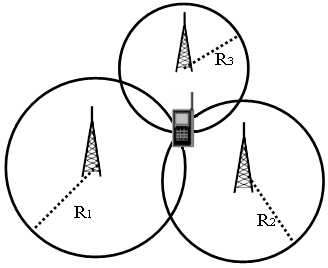
\includegraphics[width=1\textwidth]{time_of_arrival}
				\caption[Time of arrival]{A distance from the receiver to each transmitter is determined using known signal velocities and measured time differences. Trilateration of these distances yields position. (intechopen.com)}
				\label{fig:time_of_arrival}
			\end{figure}
			
			Time of arrival (or time of flight) is the travel time of a radio signal from a single transmitter to a single remote receiver. The basic observable is change in time. A distance can be directly calculated using the known propagation velocity of signals with the basic observable of change in time. Location can then be determined using multi-lateration, this requires a setup of at least one receiver and three transmitters or vise versa.
			Required with such systems is the synchronization of clocks between receivers and transmitters in order to correctly determine the propagation time of the signals from node to node.
			A significant pitfall of time of travel systems is that they suffer greatly from effects such as multi-path in which signals are reflected off nearby objects and sensed multiple times.
			\cite{k._pahlavan_wideband_1998}
			
			Figure \ref{fig:time_of_arrival} demonstrates the concept of time of arrival. The figure shows three transmitters with a single receiver in the centre of the transmitters. A radius is determined for each transmitter by calculating a distance using the known propagation velocity and measured change in time (received time - transmitted time). Tri-lateration is then used to determine a unique location of the receiver.
		
		\subsubsection{Received signal strength indication}
			\begin{figure}[H]
				\centering
				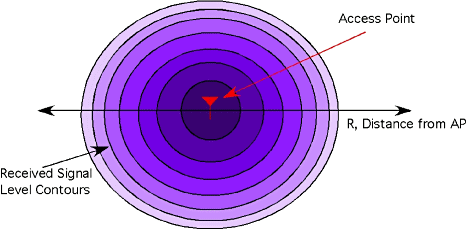
\includegraphics[width=1\textwidth]{rssi}
				\caption[RSSI]{Received signal strength indication is used to estimate a distance from a transmitter. (sensorsmag.com)}
				\label{fig:rssi}
			\end{figure}
			Received signal strength indication (RSSI) is a measure of the power level received by a sensor. Distance can be approximated between a transmitter and receiver based on the relationship between the transmitted and received signal strength. As the distance increases between a receiver and transmitter, the received signal strength diminishes (attenuation). The relationship between signal strength drop off and distance from transmitter is known. The combination of the known signal drop off relationship and the sensed signal strength allows for the determination of distance from the transmitter. Multi-lateration can then be used to determine the location of a receiver.
			A downside to this technique is that the relationship between received signal strength and distance has to be predetermined and precisely known and this often requires mapping by hand.
			
			Figure \ref{fig:rssi} illustrates the principle of RSSI. Received signal levels decrease radially from the transmitter (assuming no interference from other objects).
		
		\subsubsection{Angle of arrival}
			\begin{figure}[H]
				\centering
				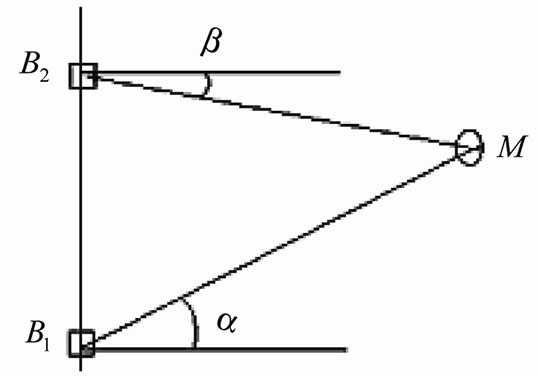
\includegraphics[width=1\textwidth]{angle_of_arrival}
				\caption[Angle of arrival]{Angle of arrival works by using a sensor array to determine the angle of arrival of incoming radio signals (http://etutorials.org/)}
				\label{fig:angle_of_arrival}
			\end{figure}
			The principle of angle of arrival works by determining the angle from which a signal is received at a receiver, transmitted from a transmitter who's position is known. The angle of arrival is typically determined using the time difference of arrival between multiple antennas in a sensor array. Position is determined using multi-angulation from readings from multiple transmitters.
			Angle of arrival systems also suffer from effects such as multi-path.
			
			Figure \ref{fig:angle_of_arrival} illustrates the principle of angle of arrival. In the figure, $B_1$ and $B_2$ each represent a transmitter. Their signals are detected by the receiver, M.
			
	\subsection{Applications of radio technologies}
		\subsubsection{Wi-Fi based systems}
			Wi-Fi based technologies are based on measurements such as time of arrival (TOA), time difference of arrival (TDOA) and direction of arrival (DOA). A pitfall of these techniques is that they are severely impaired when line of sight is not achievable. 
			These techniques also suffer due to objects such as walls and floors which attenuate and reflect signals, directly affecting accuracies.
		
			An alternative Wi-Fi based geolocation method has been explored which makes use of relative signal strengths between transmitters and receivers. Instead of measuring the time or angle of received signals, the received signal strength is measured. This negates many of the above mentioned deficiencies as the received signal strength can be mapped out in order to improve accuracies and reliability. A similar system has been employed by animal trackers with directional antennas.
			\cite{yongguang_chen_signal_2002}
	
		\subsubsection{Blue-tooth systems}
			Blue-tooth positioning works by using proximities, as opposed to angulation or lateration. As such, exact locations are not attainable using this technology. Instead, the system acts more as a geofence and works by determining which node a device is currently connected to in order to determine the location of the device. Nodes typically do not have a great range and so in order to provide location services for an entire building, many nodes will need to be purchased and set up which has a high cost associated with it.
		
			Apple has developed a protocol called iBeacon. This iBeacon protocol makes use fo Blue-tooth proximity techniques in order to enable smart devices to perform actions when in close proximity to a particular iBeacon. For example, when a blue-tooth device is placed near a kettle, the kettle will sense the presence of the phone and automatically switch on and boil the water.
			\cite{_everything_????}
		
		\subsubsection{Choke point concepts}
			\label{choke_points}
			Choke point systems work by locating and indexing tagged objects in order to track them. The concept works by passing tagged objects though a choke point (or gate), the choke point will then have a sensor which detects the tagged object passing through the gate. These systems are only able to determine when a tagged object has passed through a choke point, and so rely on deducing an objects position based upon the choke points that object has passed through.
			Many choke point sensors work with passive radio-frequency identification (RFID).
			\cite{reza_investigation_2008}
		
		\subsubsection{Grid concepts}
			Grid concepts employ a dense network of low-range receivers arranged in a predefined known pattern or layout. A tagged object within the grid will be sensed by only a few nearby receivers. By determining which receivers and tag is sensed by, a rough approximation of the location of the tagged object can be made. The tag would typically be a radio frequency identification (RFID) chip as with the choke point concepts described above in the section above.
		
		\subsubsection{Others}
			Various other radio based systems exist but will not be discussed further. These include systems based on ultra-wide band (UWB), infra-red (IR), visible light communication, as well as ultrasound technologies. All of these systems are common in that they are based on the principles described above in section \ref{radio_principles}.
	
	\section{Non-radio technologies}
		Non-radio technologies which can be used for indoor positioning will be discussed in the subsections below. These systems can provide increased accuracy at the expense of increased costs of equipment as well as installation costs.
	
	\subsection{Magnetic positioning}
		Magnetic positioning takes advantage of the way iron in buildings affects the Earth's magnetic field. The iron in the buildings creates local variations in the Earth's magnetic field which can then be sensed by compasses to map indoor locations. These local variations are mapped which then allows devices equipped with a compass to navigate and determine their locations within the indoor environment.
		\cite{supreeth_sudhakaran_geospatial_2014}
		
		Indoor Atlas is a company which provides an indoor mapping service which makes use of these local variations of Earth's magnetic field. The company provides a mobile application which enables a user to map out a particular building, and allows users to navigate the created map.
	
	\subsection{Inertial measurements}
		Inertial measurement units (IMUs) can be carried by an object in order to track the objects path through space. IMUs measure acceleration and orientation along three orthogonal axis using accelerometers and gyroscopes. Position can be determined by double integration of the acceleration measurements - this is a form of dead reckoning.
		
		Dead reckoning is the process of calculating ones current location by using previously determined positions with estimated speed and orientation over time. This yields relative position estimations. 
		
		Dead reckoning is subject to what is known as drift which is an accumulation of errors. Due to the susceptibility of IMUs to drift, they are often used in conjunction with other positioning systems such as GPS in order to correct for this drift.

\newpage
\chapter{Method}
	There are two main requirements for this alternate indoor positioning method. The first requirement is a 3D model of an environment. The second requirement is a photograph of a scene within that environment. The premise is that the photograph can be related to the 3D model in order to determine where the photograph was taken within that 3D model, thus locating the photographer.
	
	For example, consider a hypothetical building with two rooms, A and B. A person standing in one of the two rooms would like to know which room they are standing in. The person takes a photograph of the room they are in. This photograph will then be compared against a 3D model in order to determine where the scene captured in the photograph exists within the 3D model.
	
	The comparison of the photograph against the 3D model presents a problem. The problem is that the photograph and  3D model are not intrinsically comparable. So how does one compare an image to a 3D model? One solution to this problem is to create renderings throughout the 3D model and compare these renderings to the photograph. These renders are themselves images and so this permits the use of advanced and robust image recognition software to perform the matching. The focus of this paper is on the comparison of the photograph to the 3D model using image recognition software.
	
	In the following sections, the processes of creating a 3D interior model, taking a photograph and comparing a photograph to renders of the 3D model will be discussed in detail.
	
	\section{Photograph}
		In this alternate indoor positioning system, a photograph will be taken by a person or object who wishes to know their location within an indoor environment. This indoor environment will have an associated 3D model. The photograph will typically be taken from a mobile device such as a smart phone or tablet.
	
	\newpage
	\section{The 3D model}
		3D modelling can be described as the process of developing a mathematical representation of a three dimensional space using specialized computer software. The product of this process is called a 3D model. 
		
		\begin{figure}[H]
			\centering
			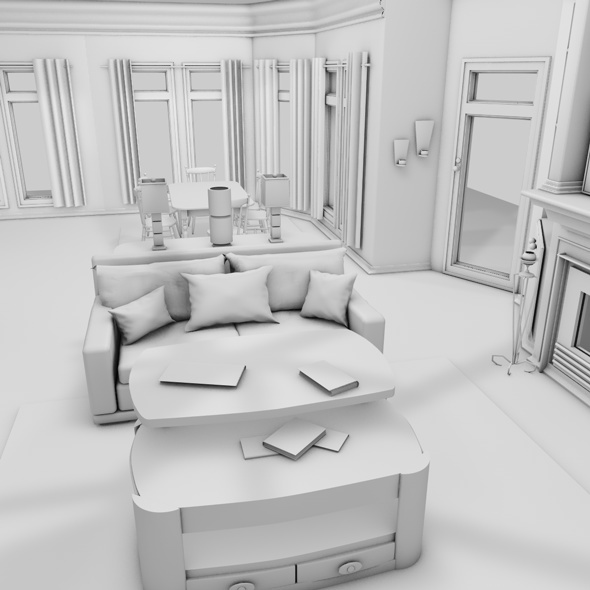
\includegraphics[width=1\textwidth]{3d_interior_model}
			\caption[3D interior model]{A 3D interior model of a sitting room.(homecg.com)}
			\label{fig:3d_interior_model}
		\end{figure}
		
		A 3D model can be visualized as a two dimensional image through a process called 3D rendering. It is this two dimensional image representation which is utilized in order to perform the comparison to a photograph in this alternate indoor positioning system.
		
		\begin{figure}[H]
			\centering
			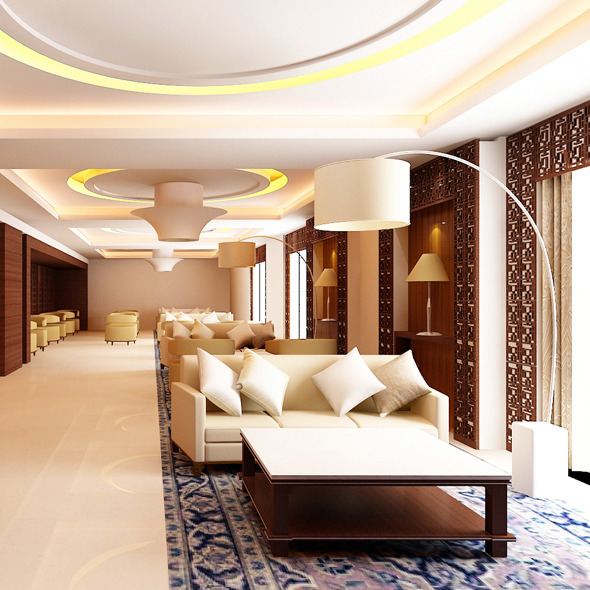
\includegraphics[width=1\textwidth]{rendered_3d_model}
			\caption[3D interior model]{A rendered 3D interior model of a sitting room.(3docean.net)}
			\label{fig:rendered_3d_model}
		\end{figure}
		
		In the subsections to follow, the process of creating a 3D model and associated renderings will be discussed and detailed.
		
		\subsection{Creating a 3D model}
			3D models can be created automatically or manually. Examples of automatic techniques include structure from motion. Manual creation of 3D models involves construction by hand using advanced computer software such as Blender. Manual creation of 3D models typically yields more detailed and accurate models. 
			In order to accurately model an existing environment, raw data such as measurements or point clouds is needed in order to serve as a basis for the model creation. The raw data serves as the initial building block and reference for the construction of the 3D model.
		
			\subsubsection{Data acquisition}
				In order to create an accurate 3D model of a building, data is required in order to aid the modelling process and serve as a template or reference for the 3D model.
				This data can come in the form of building plans, measured distances and directions or point clouds etc.
				Creating a model from building plans or other measurements involves defining model features in terms of parameters. It is often the case that the measurements or plans do not accurately reflect the real-world environment in which case the created model may contain inaccuracies when compared to the real-world case. It is for this reason that point clouds are preferable, as point clouds will more accurately represent the physical real-world environment.
				Point clouds are typically created using laser scanners.
				Creating a model from a point cloud involves creating vertices, lines and faces based on the positions of points within the point cloud. More on this in the sections to follow.
				
			\subsubsection{Data preprocessing}
				\paragraph{Cleaning laser scan point clouds}
					\subparagraph{Irrelevant points}
						During a laser scan, it often happens that a scanner captures points which are irrelevant. These irrelevant points may be points which are considered unneeded or erroneous for particular scan. Typical examples of cases leading to irrelevant points are people walking through a scan, reflections of the scanners laser beam off of surfaces, or points from objects which are generally deemed irrelevant or unneeded.
						
						\begin{figure}[H]
							\centering
							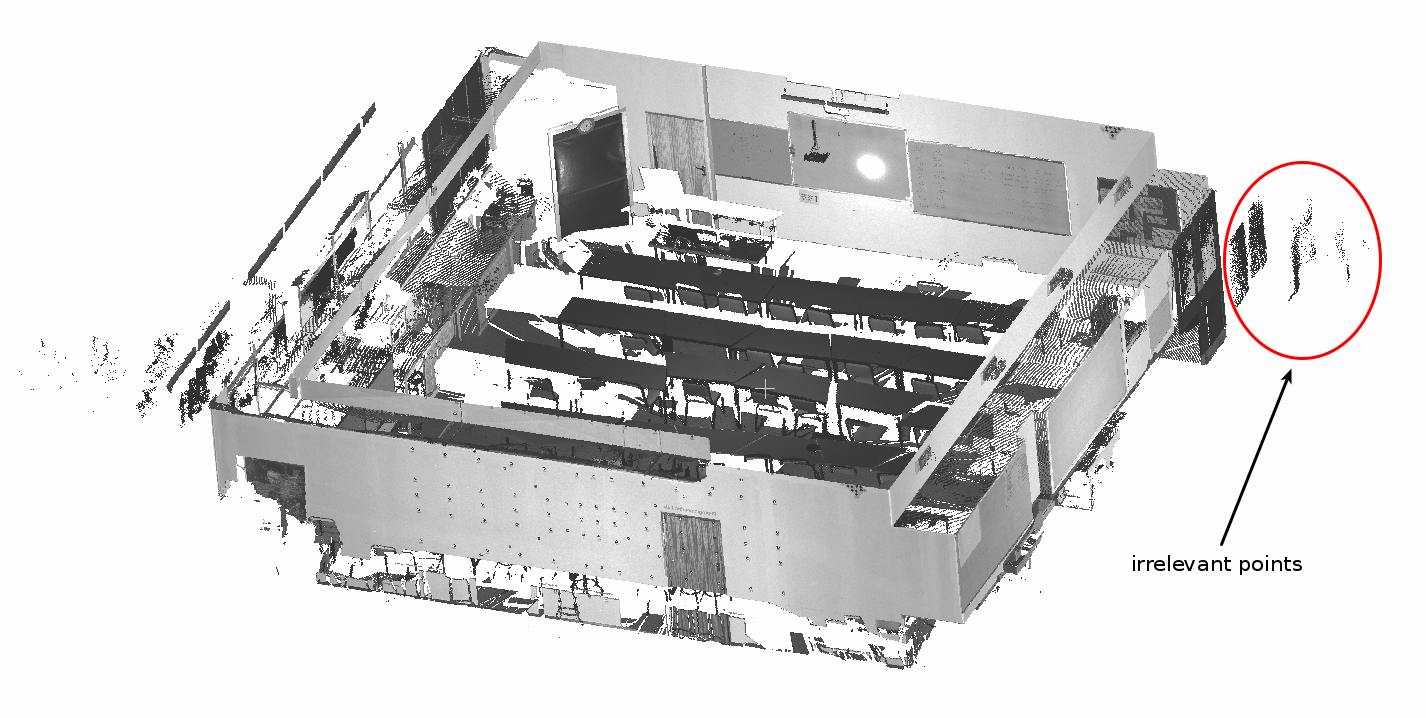
\includegraphics[width=1\textwidth]{uncleaned_point_cloud}
							\caption[Raw point cloud]{Raw point cloud containing irrelevant points}
							\label{fig:uncleaned_point_cloud}
						\end{figure}
						
						These irrelevant points need to be removed from the point cloud. The removal of irrelevant points from a point cloud is typically referred to as cleaning.
						Cleaning can be performed manually by selectively removing irrelevant points using computer software, or automatically be defining some criterion by which points which should be removed.
					
						\begin{figure}[H]
							\centering
							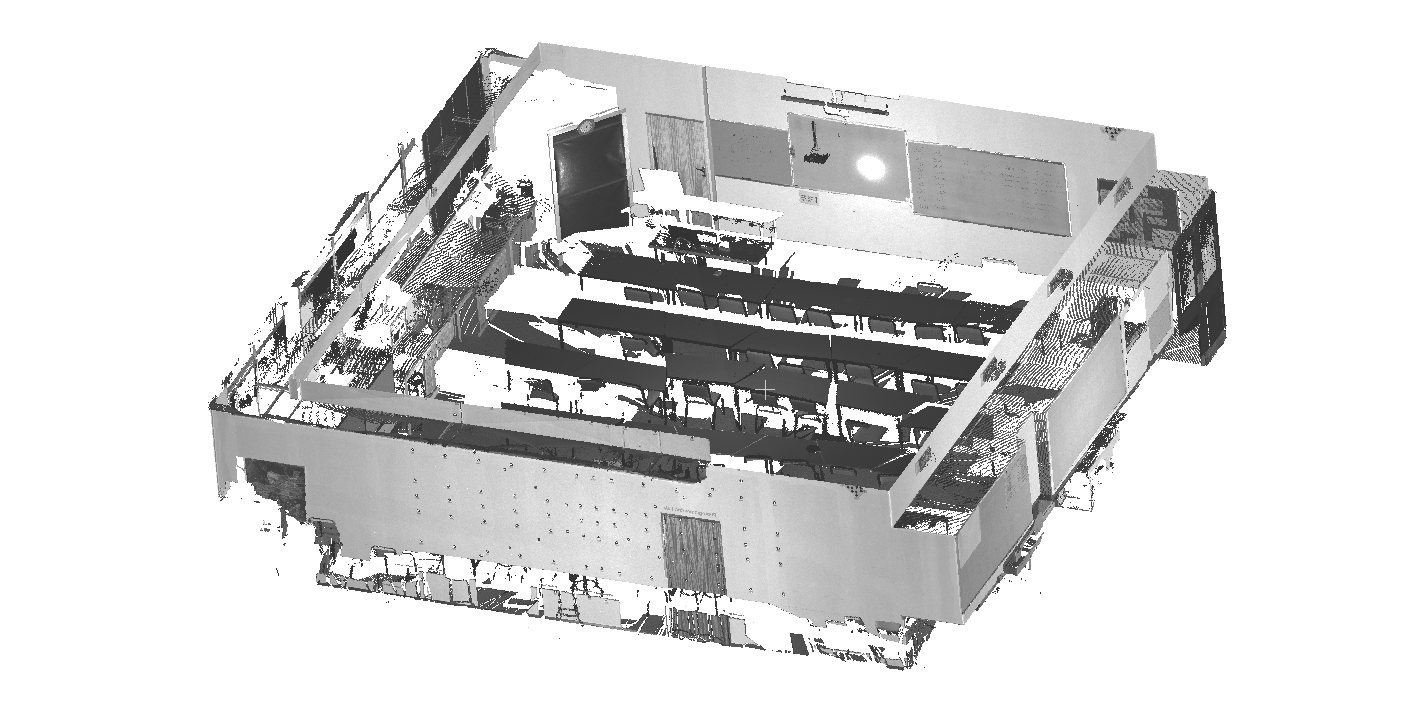
\includegraphics[width=1\textwidth]{cleaned_point_cloud}
							\caption[Cleaned point cloud]{Cleaned point cloud with irrelevant points removed}
							\label{fig:cleaned_point_cloud}
						\end{figure}
						
					\subparagraph{Down sampling}
						Due to laser beam divergence of scanners laser, points nearer to the scanner are packed more densely than those further away. The density of the points decreases radially from the scanners location.
						
						\begin{figure}[H]
							\centering
							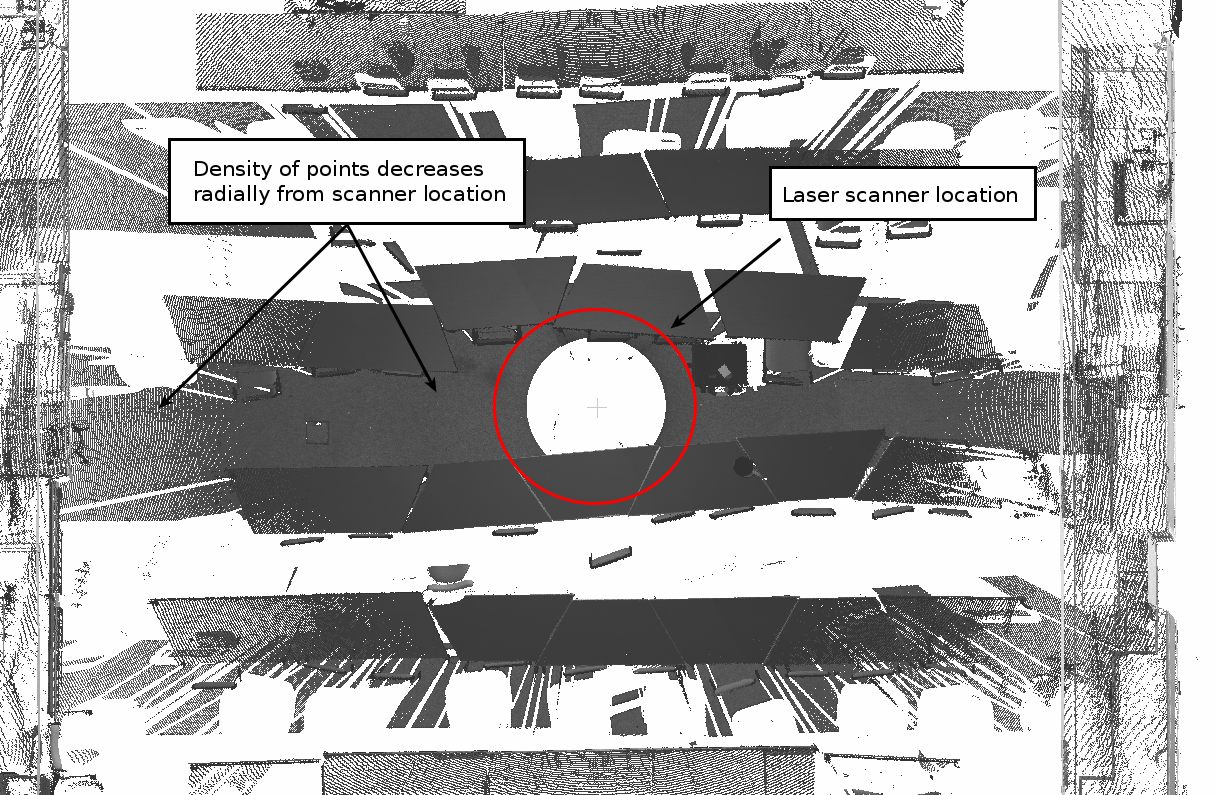
\includegraphics[width=1\textwidth]{dense_point_cloud}
							\caption[Dense point cloud]{Raw point cloud has a high point density near the location of the scanner. The point density decreases radially from the scanners location.}
							\label{fig:dense_point_cloud}
						\end{figure}
						
						Figure \ref{fig:dense_point_cloud} shows a point cloud with a high density near the scanners location. Most of the points near the scanner in the high density area are superfluous.
						
						It is often unnecessary to have the points packed at such a high density as the high density adds very little additional information to the overall point cloud. A process known as down sampling can be performed on a point cloud in order to make the point density more uniform. Down sampling works by iteratively removing points which fall within a specified distance of other points in a point cloud. The end result is that the point cloud's file size, and the computational effort required to visualize and manipulate the point cloud is greatly reduced.
						\cite{_selection_????}
						
						\begin{figure}[H]
							\centering
							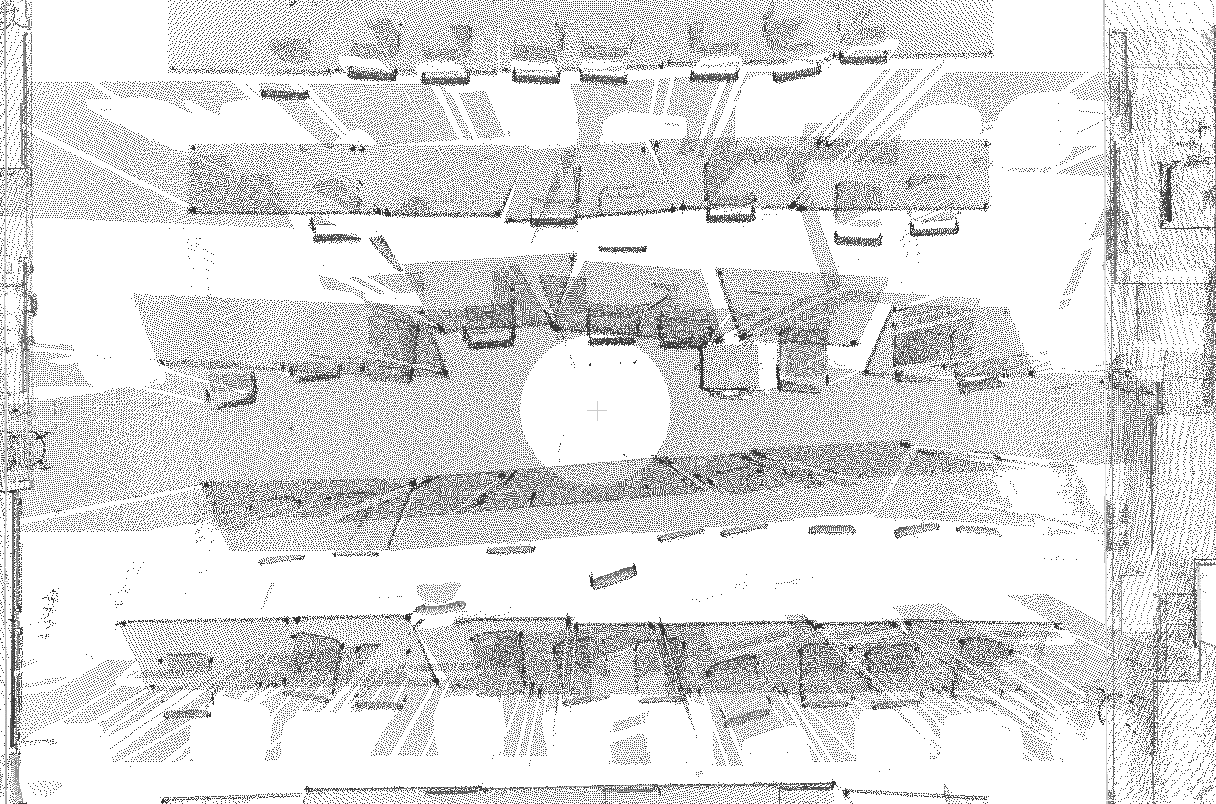
\includegraphics[width=1\textwidth]{uniform_point_cloud}
							\caption[Down sampled point cloud]{Down sampling yields a uniformly dense point cloud.}
							\label{fig:uniform_point_cloud}
						\end{figure}
						
						In contrast to figure \ref{fig:dense_point_cloud}, figure \ref{fig:uniform_point_cloud} shows a point cloud after a down sampling operation.
				
			\subsubsection{Constructing the 3D model}
				Solid modelling is a consistent set of principles for mathematical and computer modelling of three-dimensional solids which forms the foundation of computer-aided model design. 
				\cite{vadim_shapiro_solid_2001}
				3D models are created using what are known as solid representation schemes. The common aim of these solid representation schemes is to organise modelled geometric and topological data in the form of consistent data structures. A model may be created using any number of combinations of solid representation schemes. Some relevant schemes will be discussed in the sections to follow.
				
				\paragraph{Boundary representation (B-rep)}
					Boundary representation (B-rep) is a solid representation scheme which represents shapes using limits. In boundary representation, a solid is represented as a collection of connected surfaces. These surfaces are created using topological items: faces, edges and vertices. As a result of boundary representation modelling objects using limits, boundary representation lends itself to accurately modelling imperfections and inconsistencies of real-world features.
					\cite{hongxin_zhang_introduction_2007}
					\begin{figure}[H]
						\centering
						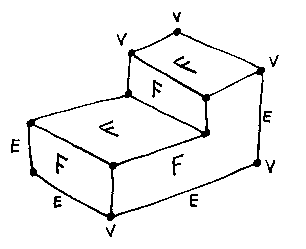
\includegraphics[width=1\textwidth]{brep}
						\caption[Boundary representation]{Boundary representation represents objects using vertices (V), edges (E) and faces (F). (homepages.inf.ed.ac.uk)}
					\end{figure}
				
				\paragraph{Constructive solid geometry (CSG)}
					Constructive solid geometry is a solid representation scheme which works by creating complex objects using boolean operators of what are known as primitive objects. Primitive objects are the simplest type of objects and are used to create more complex objects by performing operations such as unions, intersections and differences.
					\cite{foley_computer_1996}
					\begin{figure}[H]
						\centering
						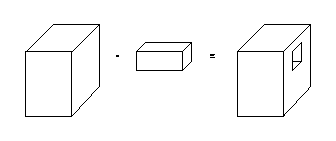
\includegraphics[width=1\textwidth]{csg}
						\caption[Constructive Solid Geometry]{Constructive Solid Geometry subtraction of two primitives to form a new object. (cadd.web.cern.ch)}
					\end{figure}
				
		\subsection{Level of detail of the 3D model}
			In terms of 3D modelling, level of detail refers to how thoroughly real-world objects have been modelled and how closely those modelled objects resemble their real-world counterparts.
			
			\begin{figure}[H]
				\centering
				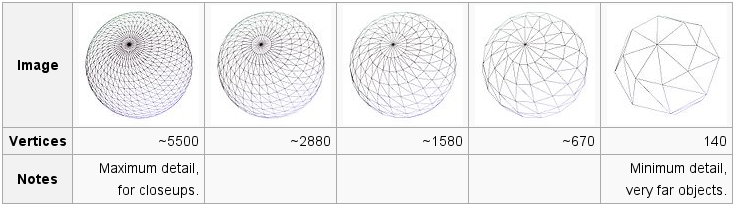
\includegraphics[width=1\textwidth]{level_of_detail_example}
				\caption[Level of detail]{Level of detail example. (www.in-ex.hu)}
				\label{fig:lod}
			\end{figure}
			
			Figure \ref{fig:lod} above illustrates the concept of level of detail. A sphere has been modelled at various levels of detail, decreasing from left to right. Models with a low level of detail are quicker to create and less computationally intensive to manipulate. High level of detail models take longer to create but increase the quality of the 3D model.
				
			\subsubsection{Lighting}
				Lighting is a very important component of any 3D model. Lighting can drastically alter the appearance of a 3D model as well as its overall accuracy in terms of how realistic it is. When creating the 3D model for this investigation, a great deal of attention was paid to lighting. Each consideration is discussed in detail in the sections to follow.
				
				\paragraph{Light source}
					When modelling light sources, there are a few considerations which need to be made, they are detailed in the paragraphs which follow.
					
					\subparagraph{Colour temperature}
						The colour temperature of a light source is the temperature of an ideal black-body radiator that radiates light of comparable hue to that of the light source. Colour temperatures are typically statued in the unit of absolute temperature, the Kelvin, with the symbol K.
						\begin{figure}[H]
							\centering
							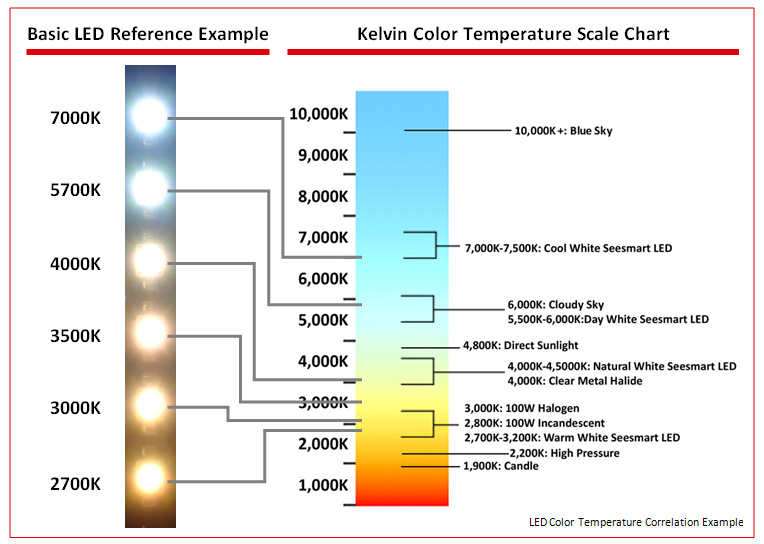
\includegraphics[width=1\textwidth]{colour_temperature}
							\caption[Colour temperatures]{Colour temperatures (seesmartled.com)}
							\label{fig:colour_temp}
						\end{figure}
						Figure \ref{fig:colour_temp} above shows how colour temperatures relate to real world conditions.
				
					\subparagraph{Position of lights}
						In order to accurately replicate shadows and intensities of real-world conditions, the light sources in a 3D model needs to be strategically placed as well as calibrated in order to best reflect the real-world conditions in terms of shadows and reflections.
						
						\begin{figure}[H]
							\centering
							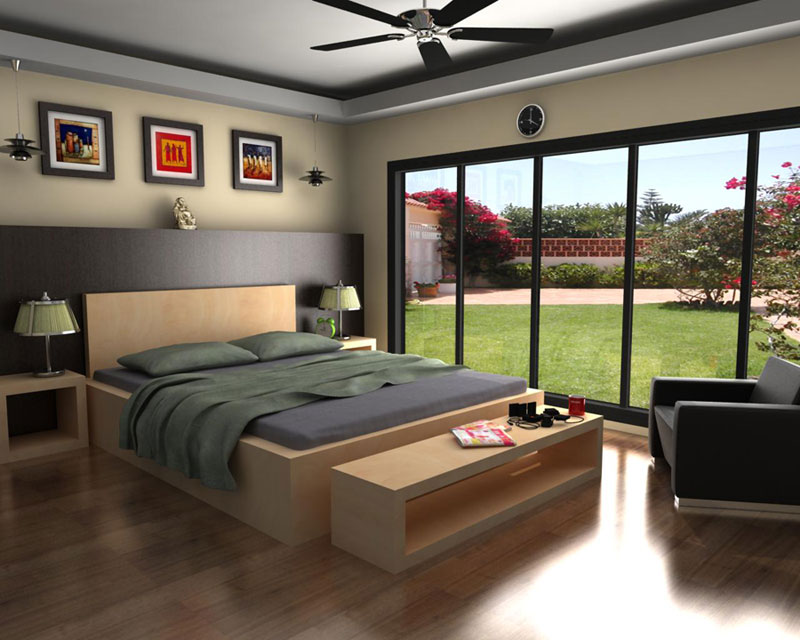
\includegraphics[width=1\textwidth]{light_glare}
							\caption[Light glare]{Notice the glare from the ambient light on the floor and head board of the bed and surrounding walls. (architecturalmodelingindia.com)}
						\end{figure}
					
					\subparagraph{Light intensity}
						Luminous intensity is a measure of the wavelength-weighted power emitted by a light source in a particular direction. In order to accurately model the real-world lighting intensities in a 3D model, each light source needs to be adjusted individually and judged by visual inspection to best model the real-world light conditions.
						
			\subsubsection{Texture}
				Surface finish, also known as surface texture or surface topography, is the nature of a surface as defined by three characteristics of lay, surface roughness and waviness.
				\cite{e._paul_degarmo_materials_2003}
				Textures are applied to surfaces in 3D models in order to accurately represent real-world textures. Textures affect the visual appearance of a surface as well as the way light interacts with that textured surface. Various texture profiles are often built into 3D modelling software. For example, pre-made textures for wood and concrete exist and can be places on floors and walls.
			
		\subsection{Renderings of the model}
			Rendering can be described as the process of generating an image from a 2D or 3D model by means of computer programs. Renders can either be generated in real-time, or pre-rendered.
			
			The software used to create the 3D model in this investigation is Blender. Blender offers three built in render engines: Blender Render, Cycles Render, and Game Render, various other render engines are available. Each have their own positives and negatives. One of the common trade offs between render engines is render time and quality.
			
			\begin{figure}[H]
				\centering
				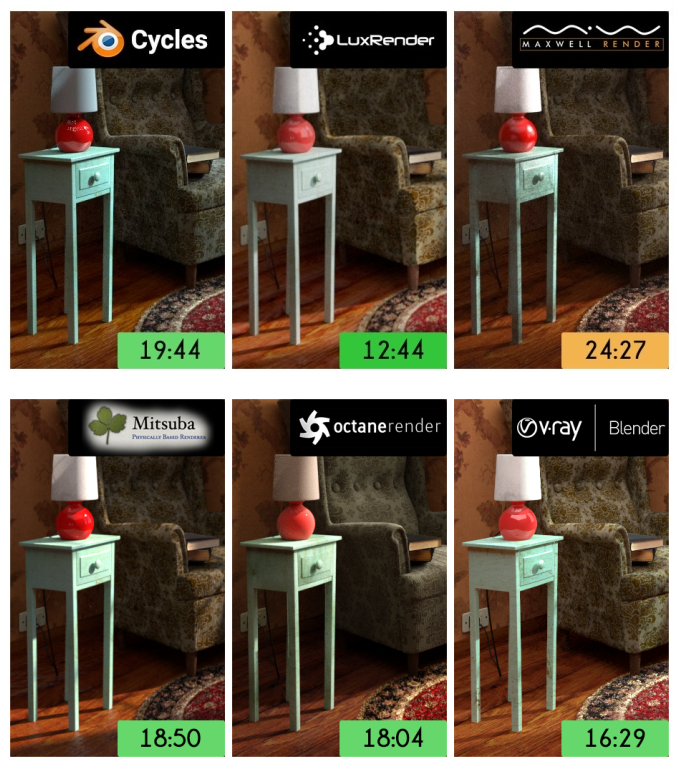
\includegraphics[width=1\textwidth]{render_engines}
				\caption[Comparison of render engines]{Six tiles showing a comparison of render engines. The name of each render engine is displayed in the top right corner of each tile. The time taken for the render to complete is on the bottom right of each tile. (blenderguru.com)}
				\label{fig:render_engines}
			\end{figure}
			
			Renders of 3D models can be created using different renderer engines, and under various different render settings. The effect of altering the render engine and settings will be a subject of investigation.
			
	\section{Comparison of the model to the photograph}
		This section deals with the comparison of the photograph to the render of the 3D model.
		
		The principle here is that there exist algorithms which, provided with a test image and query image, are able to detect the test image within the query image, yielding transformation parameters which relate the test image to the query image. These transformation parameters can be used together with photogrammetric principles to yield the location of the camera which took the photograph.
		
		\subsection{Performing the comparison}
			\subsubsection{Feature matching}
				\begin{figure}[H]
					\centering
					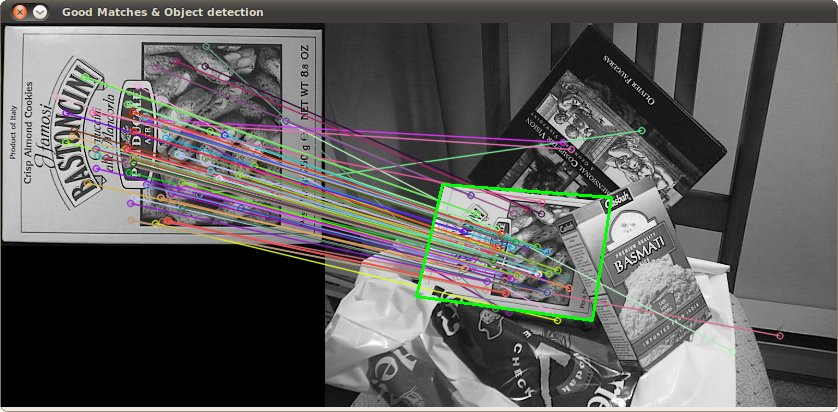
\includegraphics[width=1\textwidth]{feature_homography_example}
					\caption[Feature homography]{Feature homography (docs.opencv.org)}
					\label{fig:feature_homogrophy}
				\end{figure}
				
				Figure \ref{fig:feature_homogrophy} above illustrates the process of comparing a test image to a query image. The figure contains two images, one test image on the left side which is the cover of a rusk box. On the right is the query image. The query image is a more complex scene, which contains the test image within it. Here, the test image has been detected within the query image. An algorithm has drawn a green box around where it thinks the test image lies within the query image. This green box is defined by a transformation relating it to the test image. The process of performing the comparison will be discussed in detail in the sections to follow.
			
			\subsubsection{Key points}
				The first step involved in performing a comparison requires determining what are known as key points (or features) within an image. Key points represent specific patterns or features which are unique, can be easily tracked, and can be described and compared.
				
				To provide an example of what key points are, consider the image below:
				
				\begin{figure}[H]
					\centering
					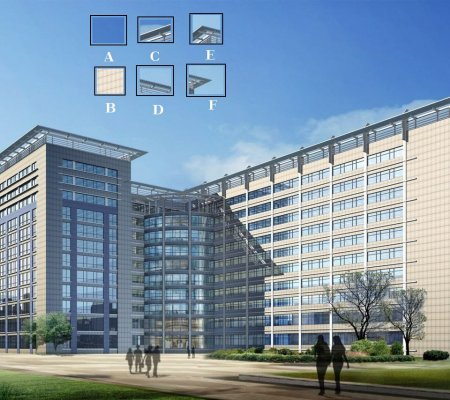
\includegraphics[width=1\textwidth]{feature_building}
					\caption[Key points]{Key point demonstration (docs.opencv.org)}
					\label{fig:feature_building}
				\end{figure}
				
				Figure \ref{fig:feature_building} is of a large building complex. At the top of the image there are six alphabetically labelled blocks. Each block contains a section of the entire image and can be thought of as a key point (feature). We now want to be able to find the exact location of these blocks within the original image. 
				Blocks A and B depict flat surfaces, they are spread over a large area within the image and so it is difficult to find an exact location of these blocks within the image, that is that there are a number of locations where these blocks could fit, so they are not unique.
				Blocks C and D are slightly better in that they are the edges of the building, they could be from anywhere along the edge of the roof of the building, but it is still impossible to pinpoint exactly where they are from.
				Blocks E and F are the corners of the building. The locations of these blocks can be exactly found and so these would be good key points as they are unique.
			
			\subsubsection{Finding key points}
				The process of finding key points in an image is called feature detection. On a high level, the process works by looking for regions within an image which have large variation when that region is moved in various directions. This process will be discussed in more detail below.
				
				Consider the image below:
				
				\begin{figure}[H]
					\centering
					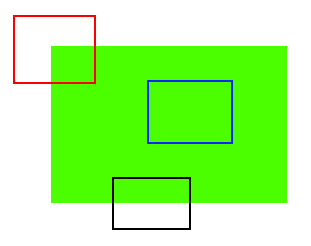
\includegraphics[width=0.9\textwidth]{feature_detection}
					\caption[Feature detection]{Feature detection example (docs.opencv.org)}
				\end{figure}
				
				In the figure above, the green rectangle represents an image and each red, blue and black rectangle represents a region for feature detection. When moving the blue rectangle vertically or horizontally by small amounts, there is no variation, the blue box still contains only green. This represents a poor feature/key point. 
				When moving the black rectangle horizontally, there is also no variation, however when moving it vertically there is (The ratio of white and green changes with this movement). When moving the red rectangle in any direction there is high variation, so this would be a good feature/key point. So corners are typically good features.
				
			\subsubsection{Describing key points}
				Once key points have been identified, they need to be described. The purpose of describing the key points is to enable the comparison of key points across different images. The idea is that a real-world point will have a similar key point description within all the images which capture the same real-world point.
				
			\subsubsection{Matching key points}
				The final step of the comparison process is that of matching key points. The concept here is that key points from separate images are individually compared against each other. If the similarity of the description of any key points exceeds some threshold, the compared key points are considered a match which would imply that they are the same real-world point.
		
		\subsection{Comparing a photograph to a 3D model}
			Now that concepts of feature detection and feature matching have been introduced, the application of the image comparison process to the objectives of this paper can be discussed.
			
			In the context of this proposed new indoor positioning technique, the test image would be a photograph that a user has supplied who wishes to know their location within an environment. The query image would be one of many renders of the 3D model of that same environment.
			
			The idea is that the test image (photograph) could be compared to a number of renders (query images) from different locations within the environment. Once a quality comparison is made, the location of the photographer can be determined using photogrammetric techniques, or by using georeferenced renders, however this is outside of the scope of this paper, however this will be further discussed in the future work chapter below.
			
			\subsubsection{Comparison metrics}
				There are two metrics which will be used to indicate the quality of a comparison. The first is that of the number of matches determined in a comparison.
				The second metric is that of the quality of the matches, in other words, how true the matches are or represent the same feature.
	
	\section{Tools}
		\subsection{OpenCV}
			OpenCV (Open Source Computer Vision) is a library of programming functions mainly aimed at computer vision. OpenCV was originally developed by Intel in Russia. OpenCV offers a large range of features and functions, including an image processing module, GUI module, camera construction and 3D reconstruction module, a 2D features framework module as well as many others. The 2D features module (features2d) was used in this investigation to facilitate the comparison of the photograph to the renders.
		\subsection{Python}
			Python is a computer programming language which was created in 1991 by a Google employee, Guido van Rossum. For this investigation, a framework was created in Python in order to facilitate the outcomes of this investigation.

	\section{Test parameters}
	\label{test_parameters}
		%TODO: This entire sections needs some attention
		There are various actions which can be performed on the model, rendered image and photograph which may influence the accuracy of, and the number of matches obtained during a comparison. These actions and their result on the accuracy of the matches are to be a subject of investigation. These actions are discussed below.
		
		%TODO: This subsection could use enumerates.
		\subsection{Model adjustments}
			\subsubsection{Level of detail}
				The level of detail of the model can be adjusted.
				
			\subsubsection{Image draping}
				Image draping can be performed.
			
			\subsubsection{Lighting}
				Lighting in the model can be adjusted.
		
		\subsection{Renders}
			Render settings can be adjusted.
			Different render engines can be used.
			
		\subsection{Image enhancements}
			A number of image enhancement processes can be performed on the photograph as well as on the rendered image. These processes will be discussed in subsections to follow.
			\subsubsection{Blurring}
				Gaussian blurring (or smoothing) is an image processing function which yields an image blurred by a Gaussian function. It is typically used to reduce noise and detail within an image. Gaussian blur acts as a low pass filter, attenuating high frequency signals.
				\begin{figure}[H]
					\centering
					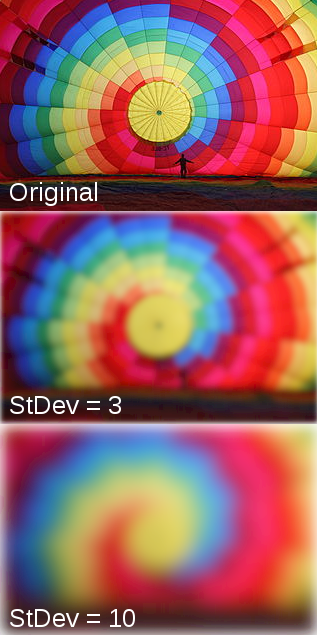
\includegraphics[width=0.6\textwidth]{gaussian_blur}
					\caption[Gaussian blur]{Gaussian blur smooths pixels in an image. (wikipedia.org)}
					\label{fig:gaussian_blur}
				\end{figure}
			
			\subsubsection{Edge detection}
				Edge detection is a method of identifying points which are discontinues, or where the brightness changes sharply.
				\begin{figure}[H]
					\centering
					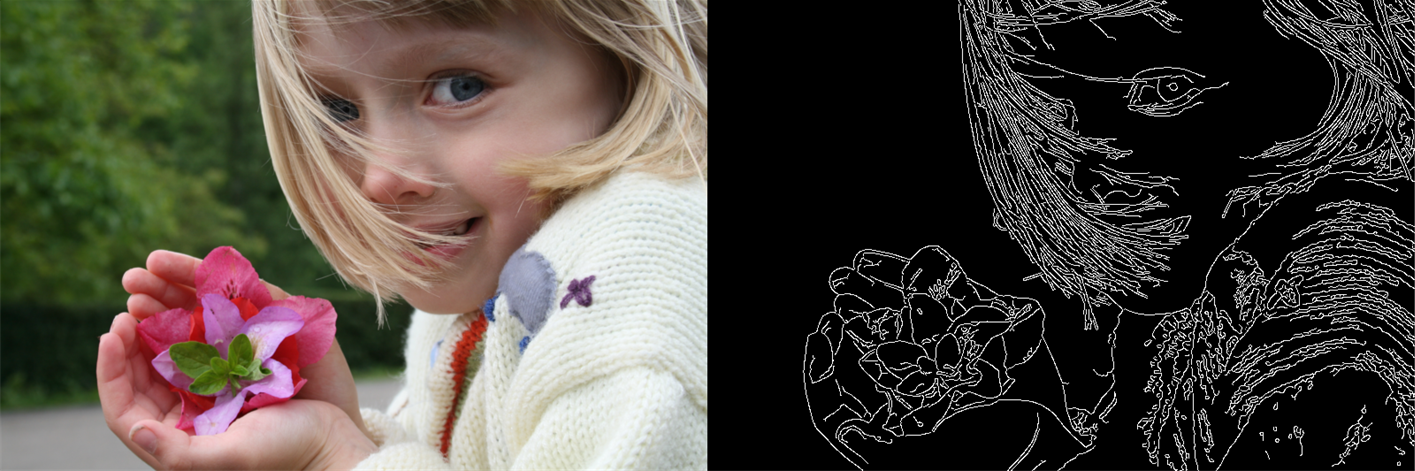
\includegraphics[width=0.9\textwidth]{edge_detection}
					\caption[Edge detection]{Edge detection highlights edges in an image. An edge represents areas in an image where there is a steep pixel value gradient. (Source: wikipedia.org)}
					\label{fig:edge_detection}
				\end{figure}

\chapter{Results}
	%TODO: This is still a bit kak.
	The Geomatics Teaching Laboratory (GTL) has been used as the subject for this investigation. Specifically the front door section of the Geomatics Teaching Laboratory was used as the basis of this investigation. The Geomatics Teaching Laboratory is located on the fifth floor of the Menzies building at UCT. The section under investigation is the south east corner of the room and was selected as there are a number of favourable features which are expected to maximize the chances of a high quality comparison, facilitating this investigation. Some of these favourable features include the whiteboard, doors, skirting, air-conditioner vents as well as the double lipped corner with a conduate running along an edge.
	
	\section{Photograph}
		The test photograph for this investigation is of the front door section of the Geomatics Teaching Laboratory (GTL). The scene consists of a air-conditioning duct on which there is a vent. On the left of the image is a section of a pin board, which contains a number of newspaper clippings. In the centre of the image is the corner of the room. The corner is relatively complex with a number of conduates running to the floor, with an electrical plug box. The blue doors are symmetrical with the exception of the bottom panels where the right hand door as a black ventilation panel. The other three panels are semi transparent glass panes which allow diffused light to enter the room.
		
		The photograph was taken using an iPhone 4S camera, which is actually an eight megapixel Sony Exmor R IMX 145.
		
		\begin{figure}[H]
			\centering
			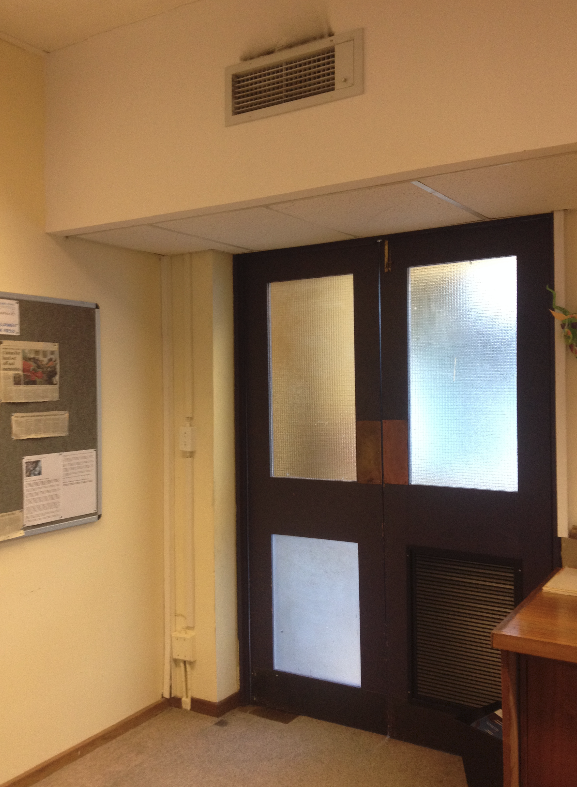
\includegraphics[width=1\textwidth]{gtl_door_area}
			\caption[GTL test image]{GTL door area which will be the subject of this investigation.}
		\end{figure}
		
	\section{3D model}
		The 3D model for this investigation was created using an open source software package called Blender. The 3D model contains the front and right walls of the GTL room, which the door section in between the two walls.
		
		\begin{figure}[H]
			\centering
			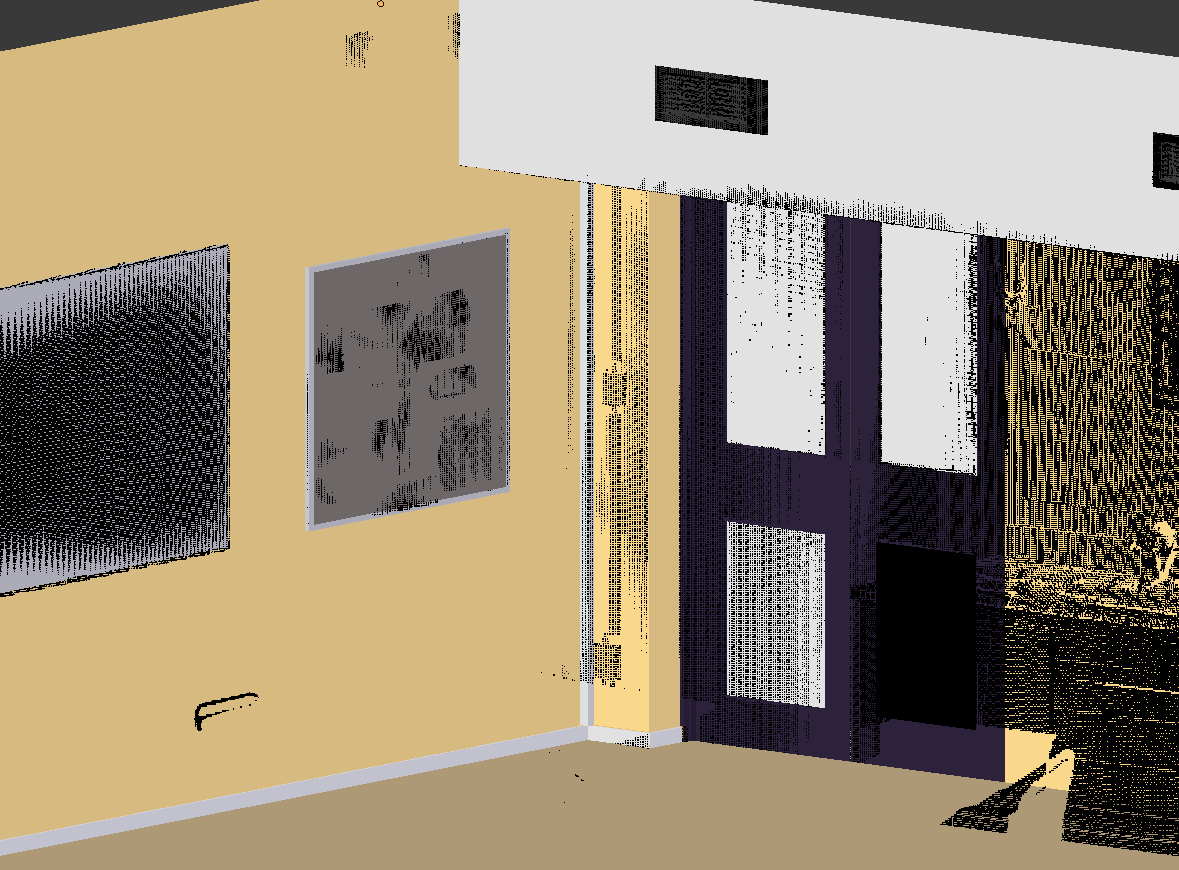
\includegraphics[width=1\textwidth]{model_with_increased_detail}
			\caption[3D model]{Focus area for this investigation. The model has been constructed using the point could (in black)}
			\label{fig:gtl}
		\end{figure}
		
		The phases involved in creating the 3D model are detailed below.
		
		\subsection{Creating the 3D model}
			\subsubsection{Data acquisition}
				In order to accurately model the scene of interest, a laser scan of GTL was conducted. The laser scanner was placed roughly in the centre of the room and a single scan was taken which captured the entire room. The scan was carried out using a ZF 5010C laser scanner at medium settings. The laser scan yielded a high resolution point cloud which would serve as the basis for the 3D model construction.
				
				\begin{figure}[H]
					\centering
					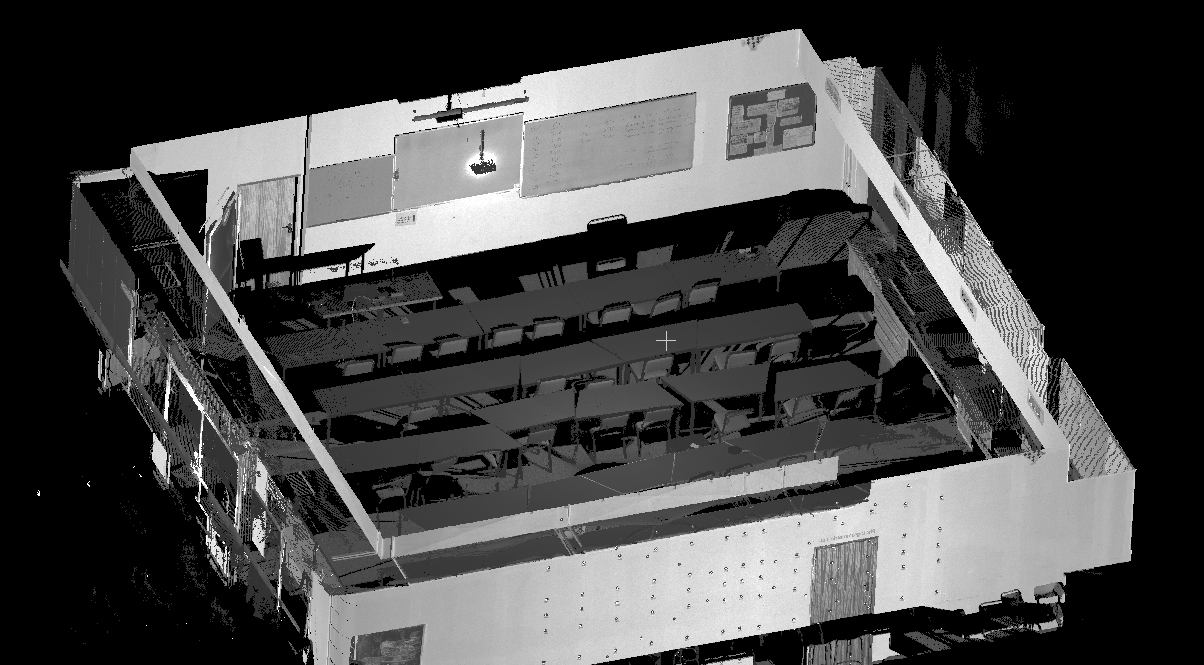
\includegraphics[width=1\textwidth]{raw_point_cloud_1}
					\caption[Raw point cloud]{Raw point cloud directly from the laser scanner.}
				\end{figure}
				
			\subsubsection{Data preprocessing}
				The point cloud was manually cleaned in a software program called CloudCompare. The purpose of cleaning the point cloud is to remove erroneous and superfluous data in order to increase the manageability of working with the point cloud.
	
				The first step cleaning the point cloud involved cutting out the sections which were not to be part of this investigation. This trivial process was performed in a software package called CloudCompare.
				
				\begin{figure}[H]
					\centering
					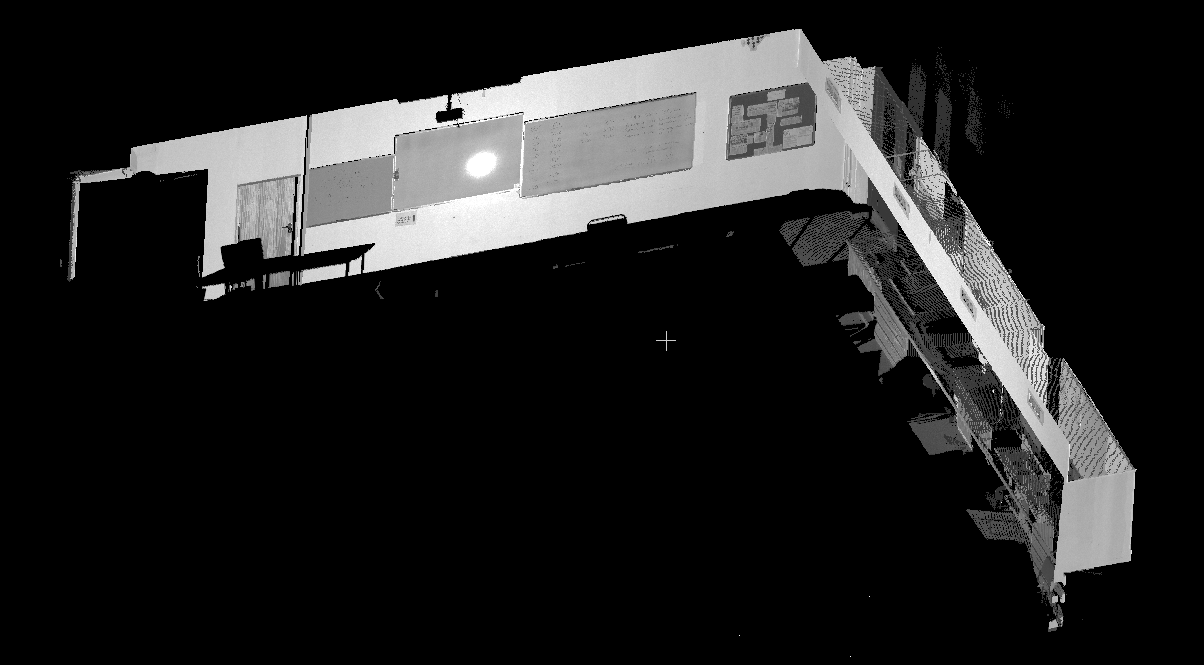
\includegraphics[width=1\textwidth]{trimmed_point_cloud_1}
					\caption[Trimmed point cloud]{Trimmed point cloud where irrelevent and uneedd points have been removed using CloudCompare.}
				\end{figure}
				
				The second step in cleaning the point cloud involved removing points which existed outside of the rooms confines, such as points outside of the glass panels of the door.
				
				%TODO: Highlight the cleaned points in the image.
				\begin{figure}[H]
					\centering
					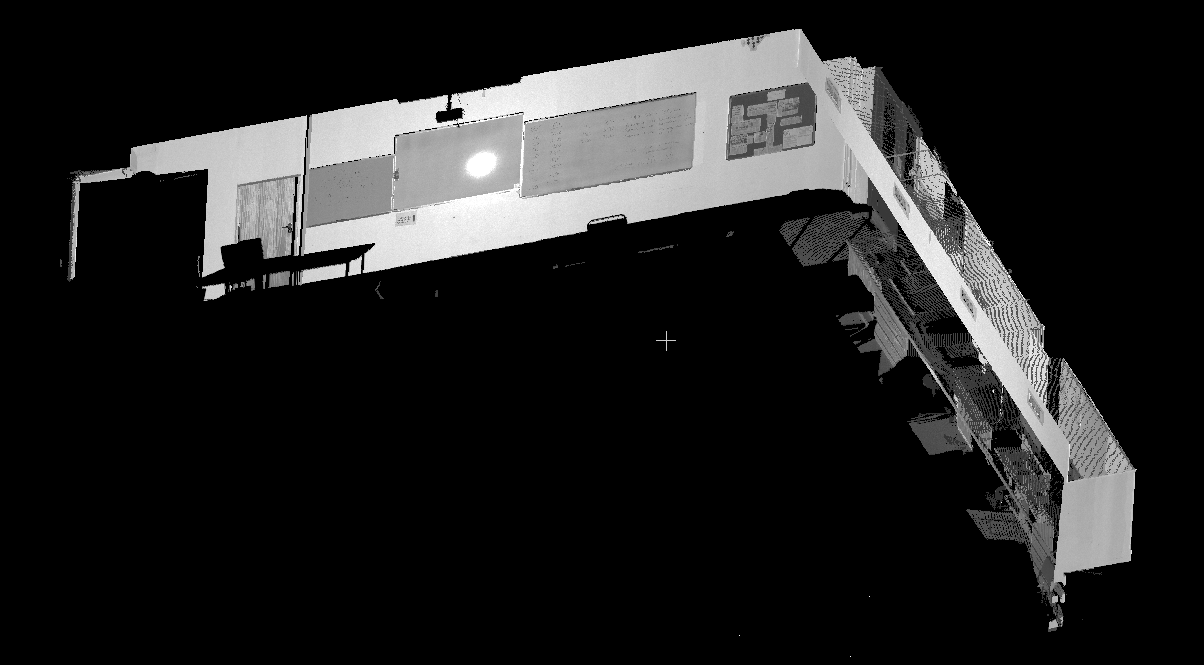
\includegraphics[width=1\textwidth]{cleaned_point_cloud_1}
					\caption[Cleaned point cloud]{Cleaned point cloud with erronous points removed.}
				\end{figure}
 
				The last step in the cleaning process involved making the point cloud uniform in density or resolution. This was done by determining the lowest resolution within the remaining section of the point cloud, this was found to be 7mm and was an acceptable resolution for use throughout the entire scene. So the entire point cloud was down sampled to a resolution of 7mm. This removed superfluous points and considerably reduced the file size of the point cloud.
				
				\begin{figure}[H]
					\centering
					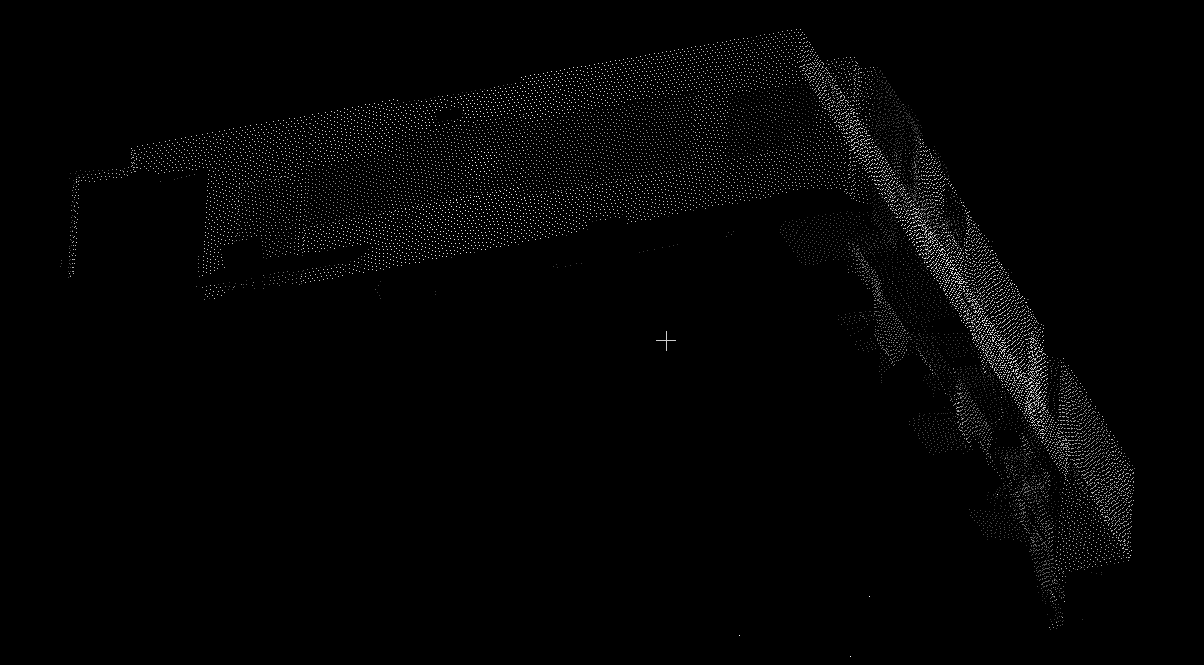
\includegraphics[width=1\textwidth]{uniform_point_cloud_1}
					\caption[Down sampled point cloud]{Down sampled point cloud with a resolution of 7mm.}
				\end{figure}
			
			\subsubsection{Model construction}
				The 3D model in this investigation was created using a solid modelling technique called boundary representation (B-rep). Boundary representation is a solid representation scheme which is a method for representing shapes using limits or edges. In boundary representation, a solid is represented as a collection of connected surfaces. The surfaces themselves are created using topological items: faces, edges and vertices.
				\cite{hongxin_zhang_introduction_2007}
				Boundary representation was selected as the solid representation scheme as it is very well suited to modelling inconsistent or imperfect objects. For example, many objects in the scene appear to be perpendicular, but upon closer inspection it can be seen that very few corners are true, and very few edges are perfectly straight. Boundary representation lends itself to accurately modelling these imperfections which leads to a 3D model which is overall more accurate, in that the model more accurately represents the real-world features.
				
				The accuracy of the model is an important consideration for this investigation. The model was constructed as accurately as possible in order to maximise the chances of obtaining good quality matches in the comparison process, and to serve as a point of further investigation (by investigating the effects of model quality/accuracy on the quality and number of matches).
				
				The software used to create and manipulate the 3D model was Blender. Blender is a free and open-source computer graphics software product. The cleaned point cloud was loaded into Blender and faces were attached to points in order to create the outline of the room, the outline consisted of the four surrounding walls, floor and ceiling. 
				
				With the extremities constructed, finer features and details were iteratively added to the model, this included the white boards on the walls, the skirting along the bottom of the walls, as well as conduates and electrical plug points, as well as the door section.
				
				\begin{figure}[H]
					\centering
					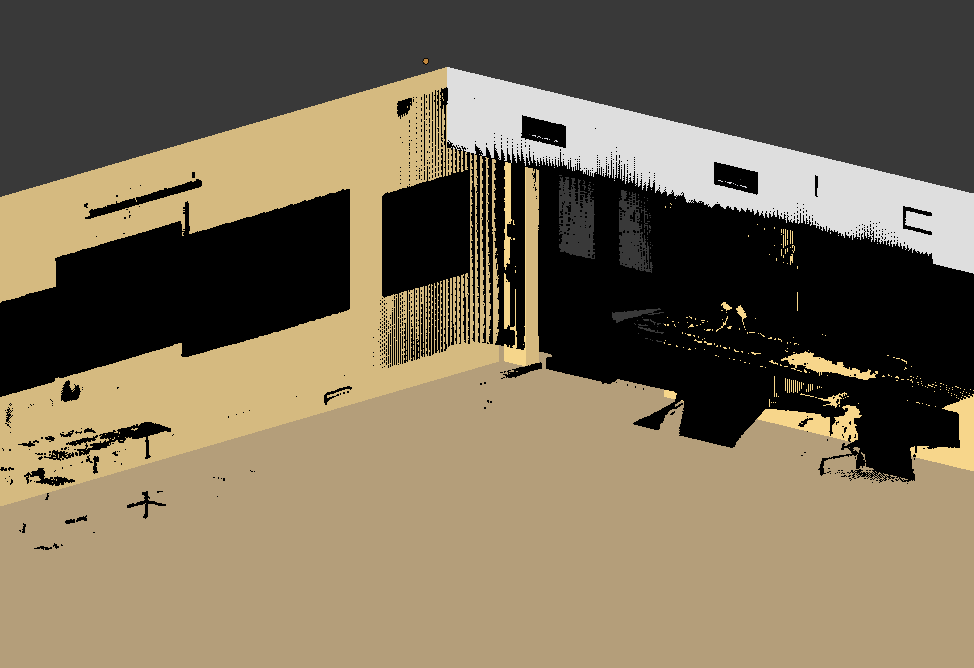
\includegraphics[width=1\textwidth]{simple_model_with_pc}
					\caption[Point cloud construction]{Walls, floor and air-conditioning duct modelled from the point cloud to form the basis of the 3D model.}
					\label{fig:simple_model}
				\end{figure}
				
				In figure \ref{fig:simple_model} the walls and floor of the room have been modelled off of the point cloud. Detail of the model was iteratively increased by modelling the finer details.
				
				\begin{figure}[H]
					\centering
					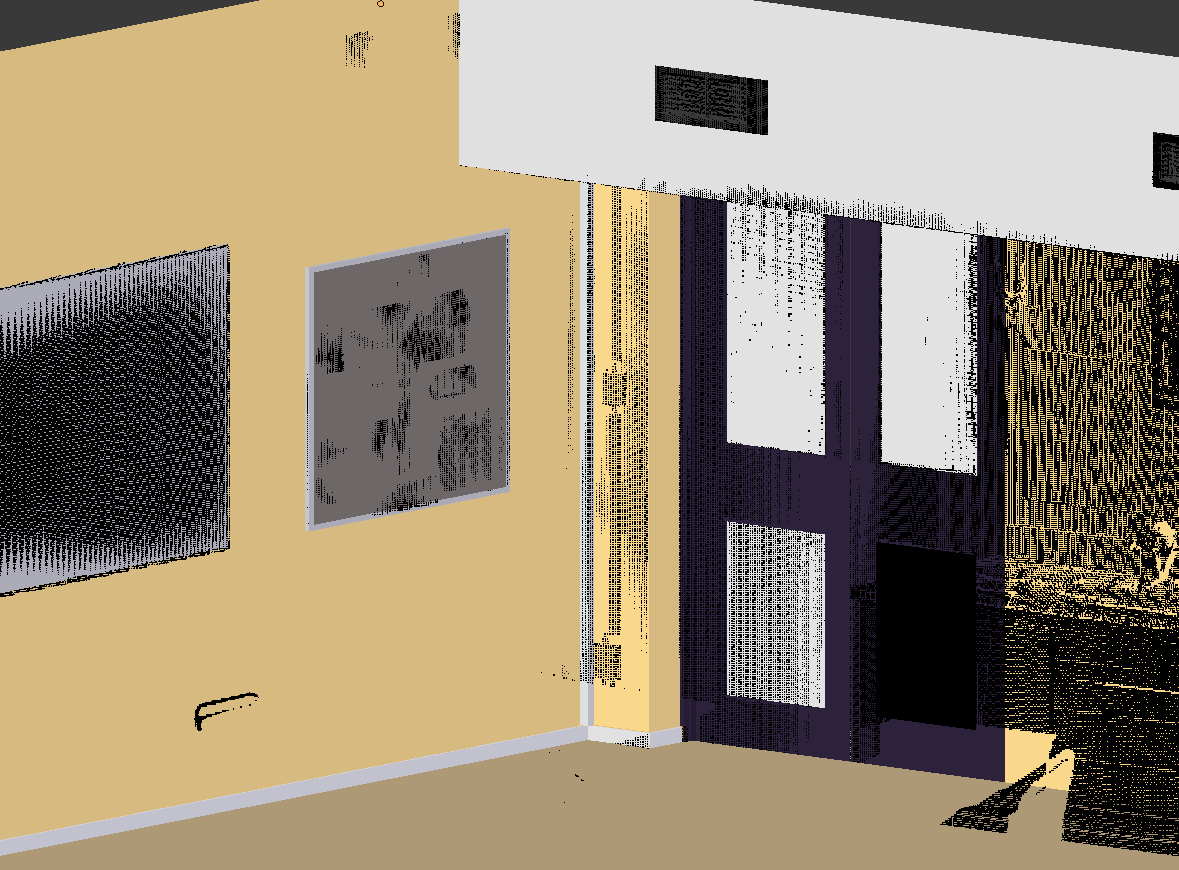
\includegraphics[width=1\textwidth]{model_with_increased_detail}
					\caption[Detailed model]{Model with increased detail including the doors, white boards and electrical conduate.}
					\label{fig:more_complex_model}
				\end{figure}
				
				Figure \ref{fig:more_complex_model} shows the model with increased detail. The skirting board, conduate, door as well as white-boards have now been added. All these features have been modelled from the point cloud and so the model is an accurate representation of the actual room in terms of scale etc.
				
		\subsection{Level of detail of the 3D model}
			\subsubsection{Objects}
				As many objects as possible have been modelled to the best possible detail. This is done in order to facilitate investigating the effects of the number of objects and the level of detail of these objects on the quality and number of matches in the comparison process. The investigation will cover multiple level of details in order to document the affect. More on this later.
				
			\subsubsection{Lighting}
				The GTL room is illuminated by florescent light panels, each containing three fluorescent tubes. The panels are rectangular with dimensions 0.5m by 1.5m. Additionally, light enters the room from the windows along the north wall, as well as through the glass panels within the door. So there are three sources of light illuminating the room.
			
				Much attention was given to the lighting within the model. This included accurately representing real-world lighting conditions within the model itself. The intensity, colour temperature and locations of light sources are all very important considerations when creating accurate 3D models.
				
				An important consideration for lighting with regards to this investigation is that lighting can vary. This includes the the variation of natural light over the diurnal cycle as well as variations due to weather conditions. Variations in artificial lighting is also an important factor, such variations include lights being switched on or off, bulbs blowing or varying brightness etc.
				
				\paragraph{Overhead lights}
					Overhead lights consisted of panels of florescent lights uniformly spaced throughout the ceiling. The each panel contained three fluorescent tubes. These light panels were reconstructed in the model and mimicked using emmisive planes subtended within a rectangle.
					
					The overhead lights have been placed in their respective real-world positions.
					\begin{figure}[H]
						\centering
						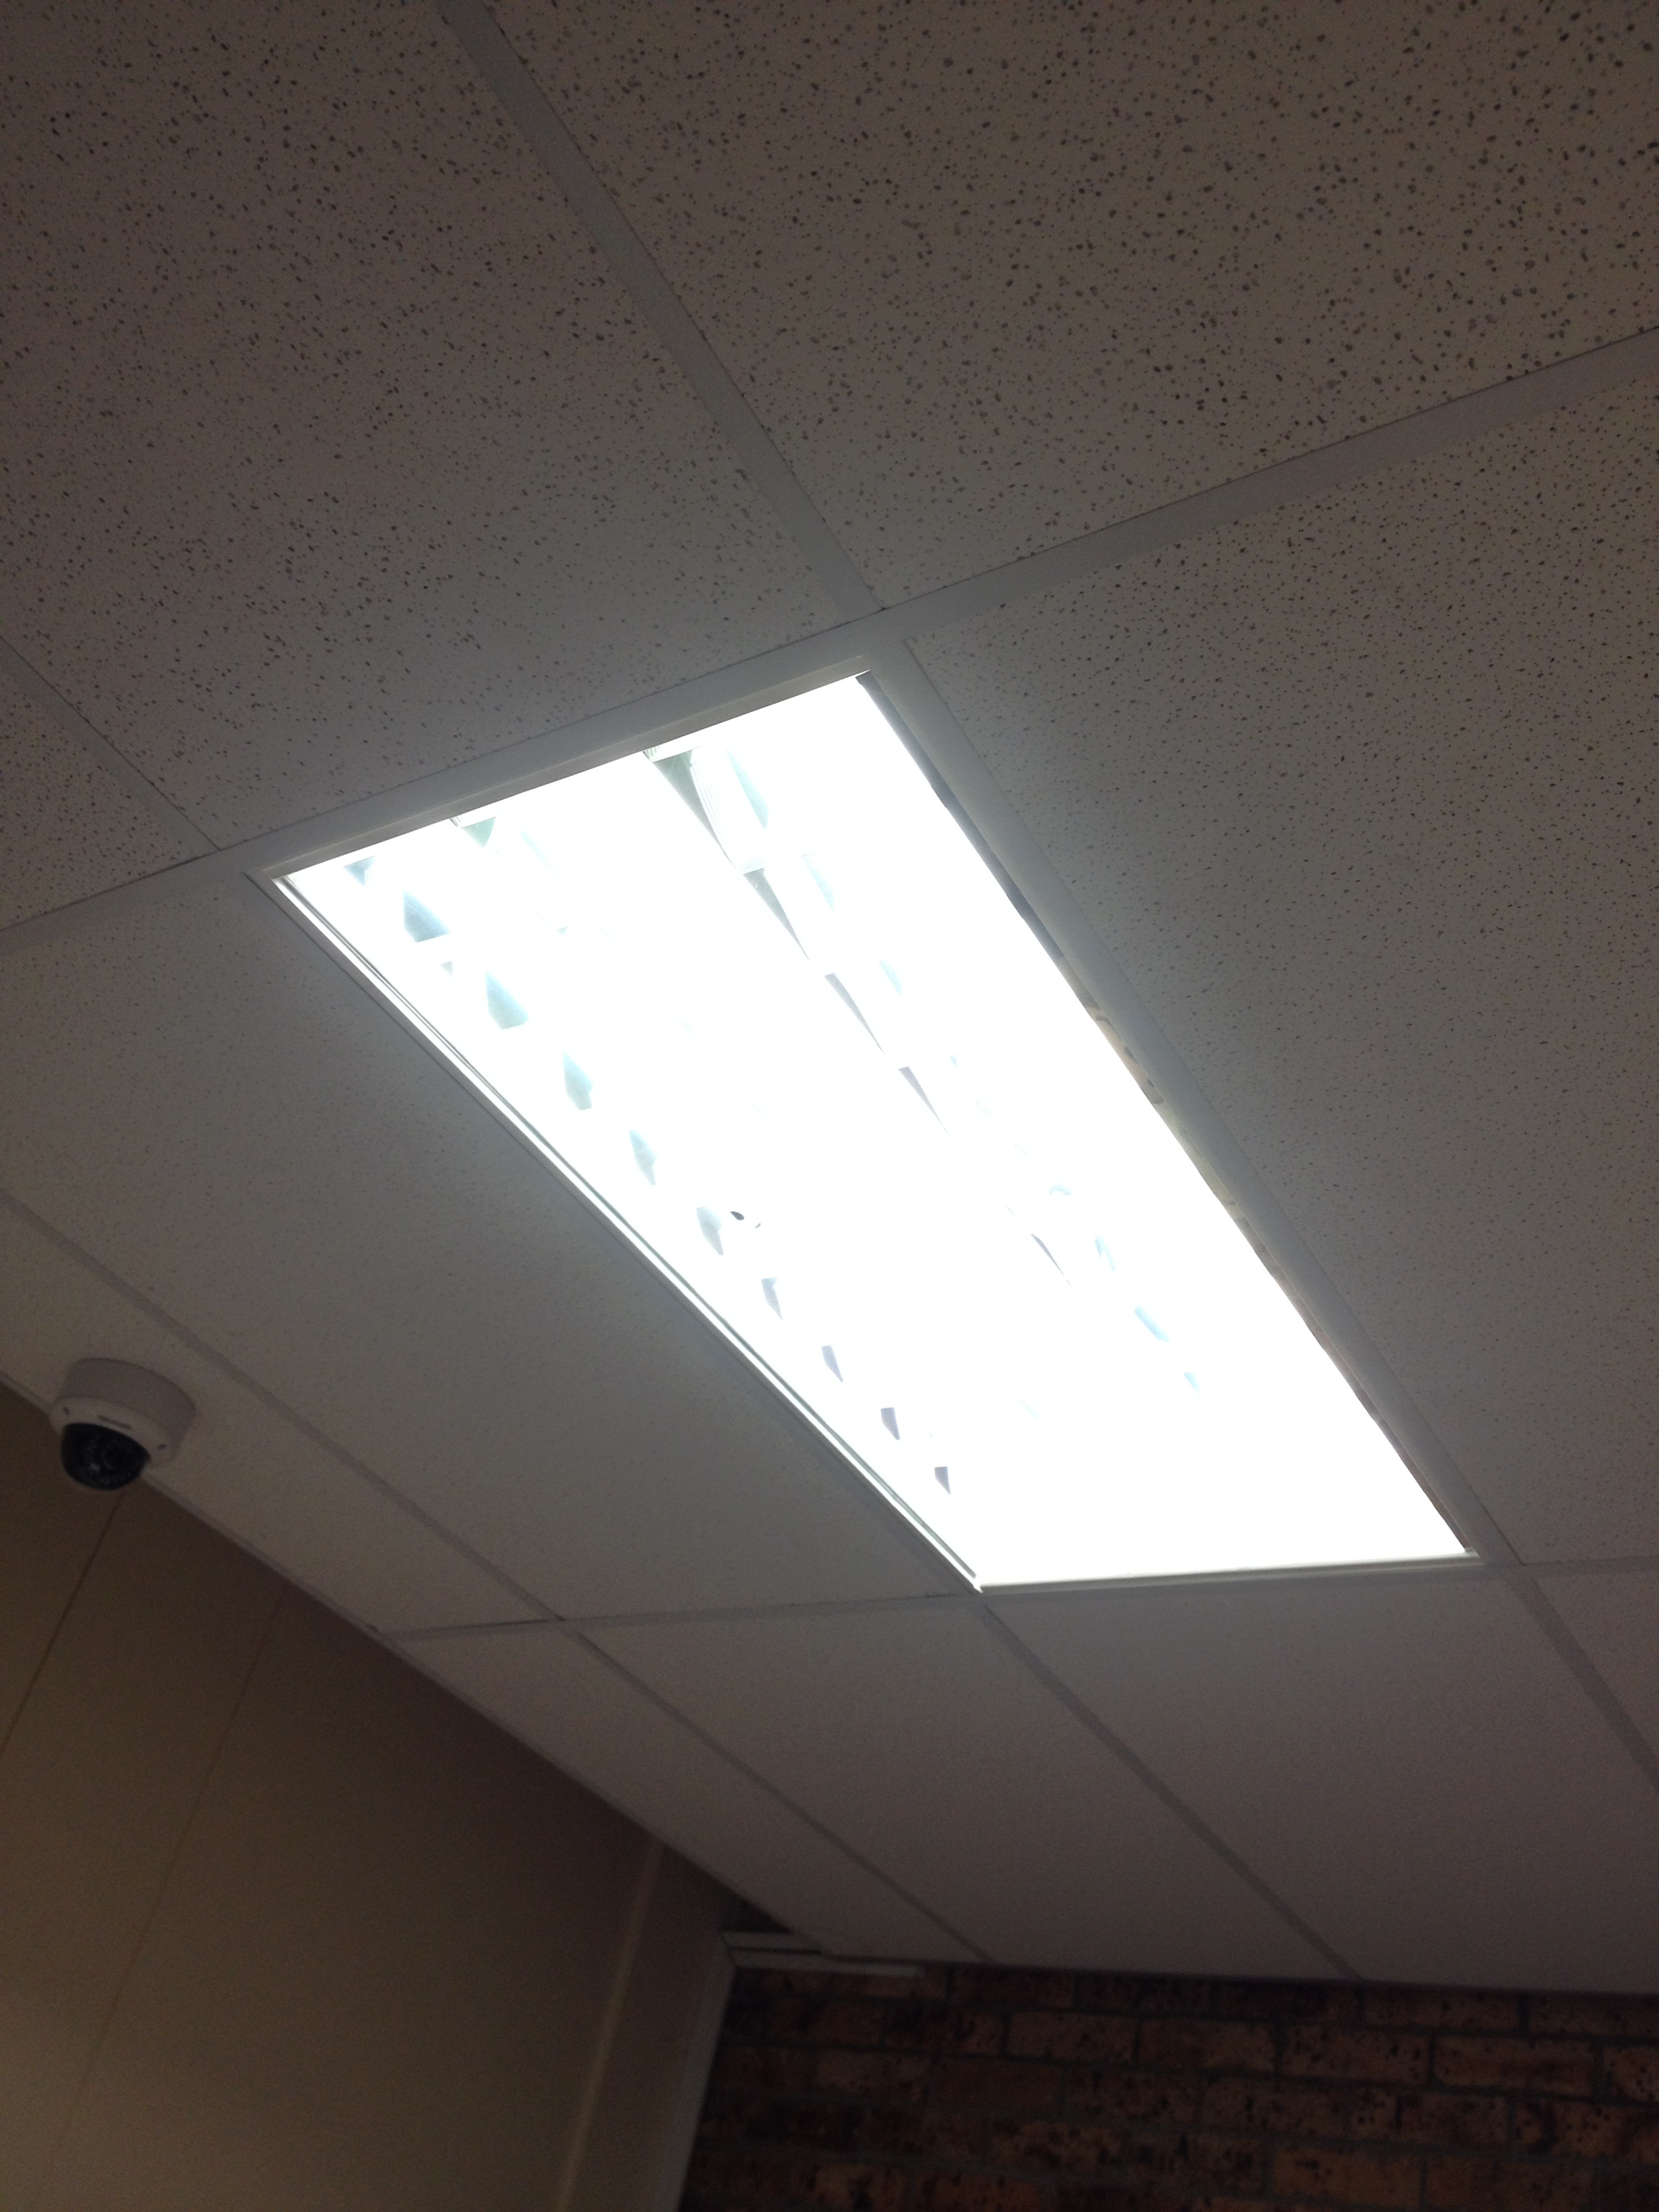
\includegraphics[width=1\textwidth]{actual_lights}
						\caption[Florescent lights in GTL]{Florescent lights in GTL.}
						\label{fig:actual_lights}
					\end{figure}
					\begin{figure}[H]
						\centering
						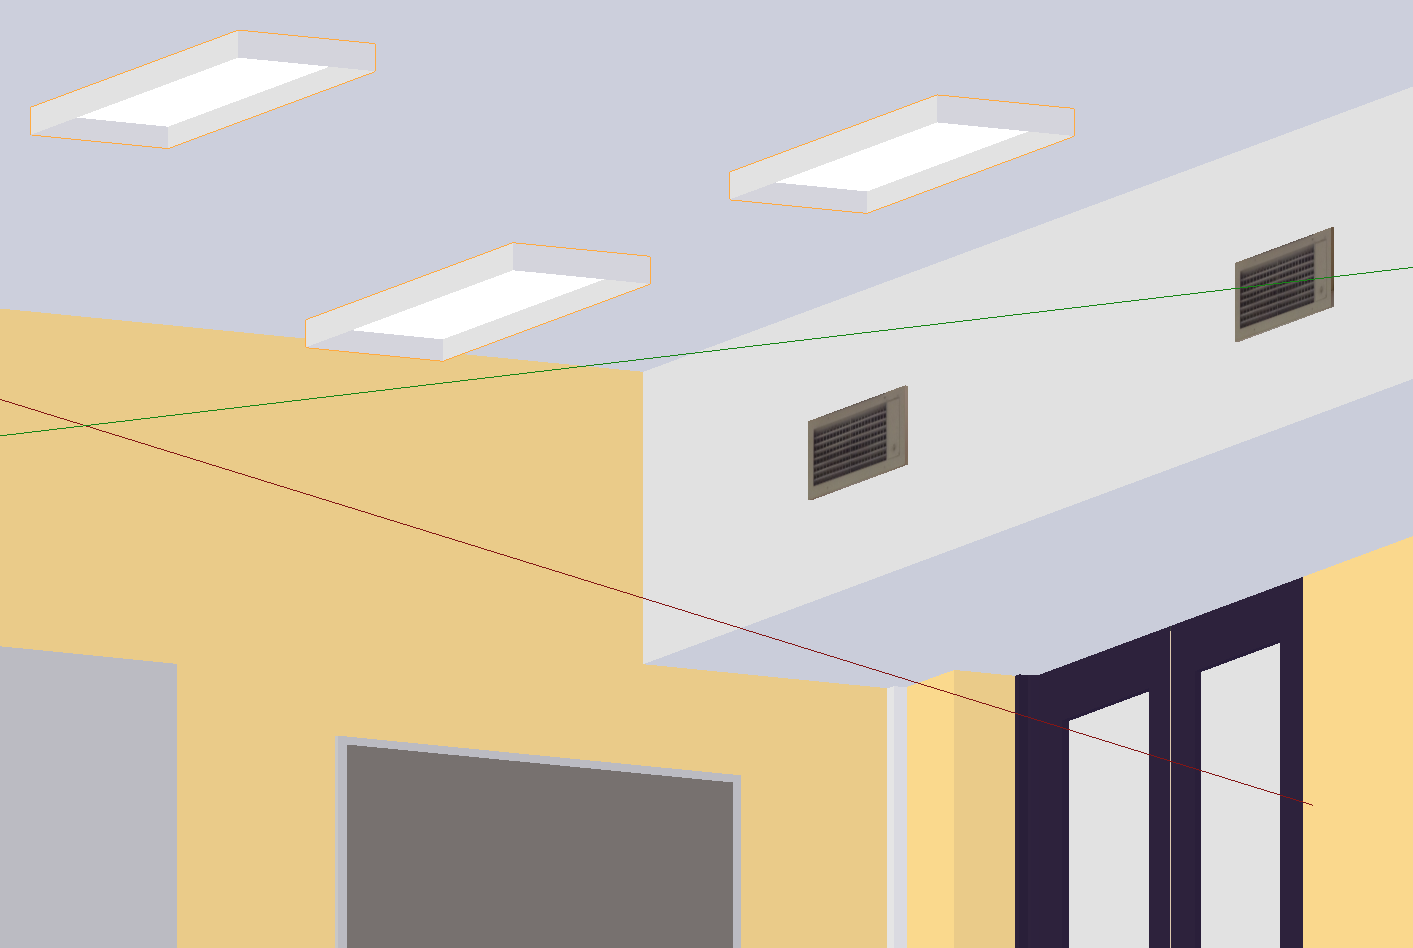
\includegraphics[width=1\textwidth]{model_lighting}
						\caption[Modelled florescent lights]{Modelled florescent overhead lights are composed of a rectangle with a subtended emmisive plane.}
						\label{fig:model_lighting}
					\end{figure}
				
				\paragraph{Natural lighting}
					In order to accurately model the natural light which penetrates though the glass panes of the door, emmisive planes were placed behind the glass panes of the door section. These emmisive planes were each calibrated in order to best represent real-world conditions of the photograph in terms of position, intensity and colour.
					
					%TODO: Add image
					{{Image of emmisive planes behind doors}}
			\subsubsection{Texture}
				Texture affects how an object interacts with light. Textures can be rough or smooth and can be arranged randomly or uniformly. Textures can reflect light specularly (mirror-like) or diffusely (randomly).
				
				\begin{figure}[H]
					\centering
					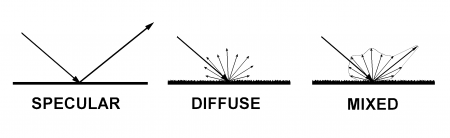
\includegraphics[width=0.9\textwidth]{light_reflection}
					\caption[Reflection]{Specular and diffuse light reflection (Source: vacuumcoating.indo)}
					\label{fig:light_reflection}
				\end{figure}
				The objects in the model have all been assigned textures in order to best reflect their real-world characteristics. The texture of objects will be another subject of investigation in this report. More on this later.
				
				%TODO: Needs work
				Particular attention has been paid to accurately representing surface characteristics of as many features as possible in the model. The glass panels in the door are set to be smooth and transparent, replicating the real-world glass panes. The texture of the walls has been adjusted so as to mimic plastered walls. The texture of the floor has been roughened to replicate the carpet. Whiteboards are smooth and glossy and the gray pin board has a rough texture.
				
			\subsubsection{Image draping}
				It is further possible to drape images of objects within the 3D model. Blender offers a feature known as UV Unwrap which enables an image to be wrapped around a modelled object. The texture of the object then becomes the image.
				
				\begin{figure}[H]
					\centering
					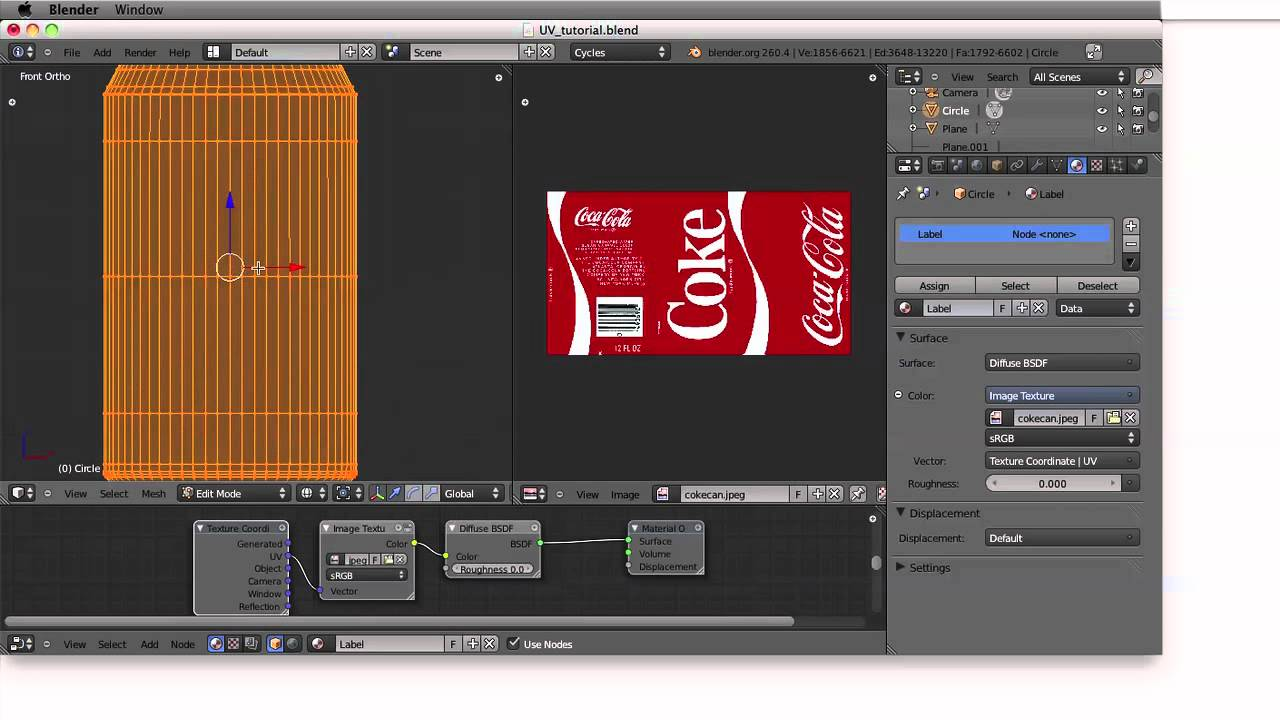
\includegraphics[width=1\textwidth]{blender_uv_unwrap_1}
					\caption[UV unwrap]{3D model is in the left pane, the right pane contains the image which will be wrapped onto the model (Source: ytimg.com)}
					\label{fig:blender_uv_unwrap_1}
				\end{figure}
				
				\begin{figure}[H]
					\centering
					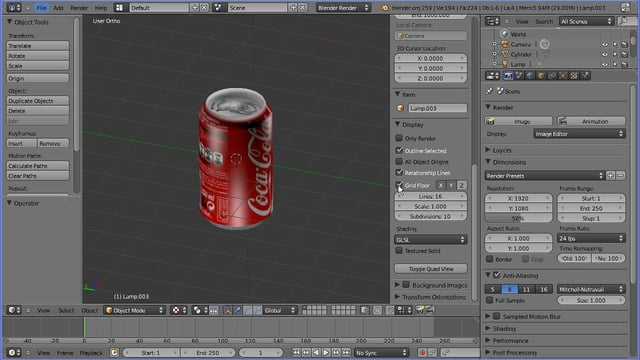
\includegraphics[width=0.9\textwidth]{blender_uv_unwrap_2}
					\caption[UV unwrap result]{The result of wrapping the model with the image (Source: vimeocdn.com)}
					\label{fig:blender_uv_unwrap_2}
				\end{figure}
				
				The affect of image draping on the quality of a comparison is another subject of investigation.
				
		\subsection{Renders}
			Renders for this investigation where created using Blender's Cycles Renderer as it provided superior render quality when compared to the standard Blender Renderer.
			
			%TODO: Needs work.
			Two render quality settings where adjusted when creating renders and were a subject of investigation. These settings pertain to the Blender Cycles render engine and affect the way light rays bounce in the 3D model. The results of altering these settings are presented in the results section to follow.

	\section{Comparing the photograph to the model}
		In order to perform the comparison between the photograph and renders of the 3D model, a testing framework has been created using the Python programming language in conjunction with the OpenCV library.
		
		The OpenCV features2d module offers various feature detection algorithms (SIFT, SURF, ORB) as well as feature matching algorithms (FLANN, BruteForce). Another OpenCV module used in this investigation was the image processing module which offers a number of image enhancement/manipulation functions which have been made use of in this investigation.
		
		\subsection{Testing framework}
			%TODO: Needs work
			In order to facilitate the investigative process, a framework was created using the Python programming language. This framework encapsulated all the various features and functions of OpenCV pertaining to this investigation.
			
			The framework has a TestCase class which encapsulates a test image, query image, a feature detection method and a feature matching method. Additionally, a TestCase encapsulates any number of image processing functions and parameters which are programmability applied to a test and or query image.
			
		\subsection{Comparison results}
			The comparison process was run a number of times with varying parameters adjusted in order to investigate and document the effects of the parameters on the quality of each comparison. The parameters which where adjusted have been discussed above in section \ref{test_parameters}. The results of these test parameters will be presented below.
			
			\subsubsection{Benchmark}
			\label{benchmark}
				%TODO: Fix comparason ambiguity
				In order to be able to qualitatively compare results of the comparison process, the best comparison result will serve as the benchmark from which results will be compared. It so happens that the best comparison result was that of comparing the raw photograph to the raw rendered image with the ORB detector and Brute Force matcher.
				
				\begin{figure}[H]
					\centering
					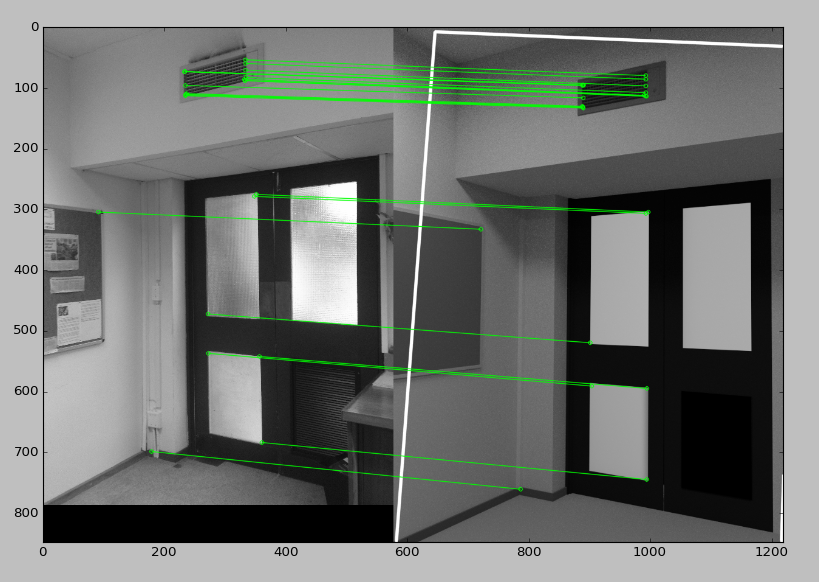
\includegraphics[width=1\textwidth]{best_comparason}
					\caption[Best comparison result]{Best comparison result.}
					\label{fig:best_comparason}
				\end{figure}
				
				The comparison result in figure \ref{fig:best_comparason} is the best attained result of all comparisons which have been made in this investigation. As such, it serves as the reference result to which all other results will be compared. The figure contains two images, the left image is the test image which in the context of this investigation is the photograph of the real-world scene. The right image is the query image and is the rendered image of the 3D model. The green circles in the images represent keypoints or features and the green lines indicate the matched keypoints between the two images. Finally, the white boundary box in the query image represents where the program thinks the test image fits into the query image. This boundary box represents a set of transformation parameters which relate the two images.
			
			\subsubsection{Photograph adjustments}
				\paragraph{Blurring}
					Blurring was performed on the test image using OpenCV's Gaussian blur function. The Gaussian blur function takes two parameters x and y which determine the magnitude of the blur along each x and y axis. The following figures show the results of the comparison using the blur along each axis on the test image.
					\begin{figure}[H]
						\centering
						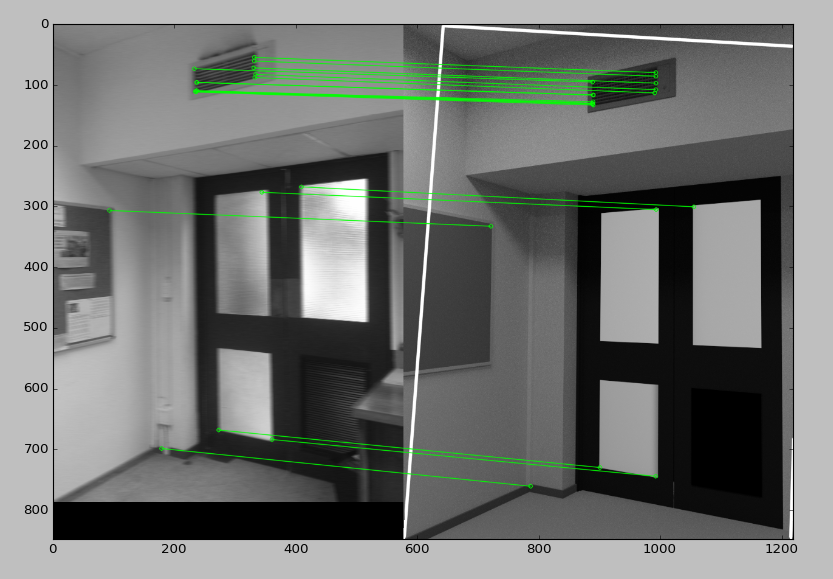
\includegraphics[width=1\textwidth]{x_blur}
						\caption{Blurring the photograph along the x axis}
						\label{fig:x_blur}
					\end{figure}
					
					\begin{figure}[H]
						\centering
						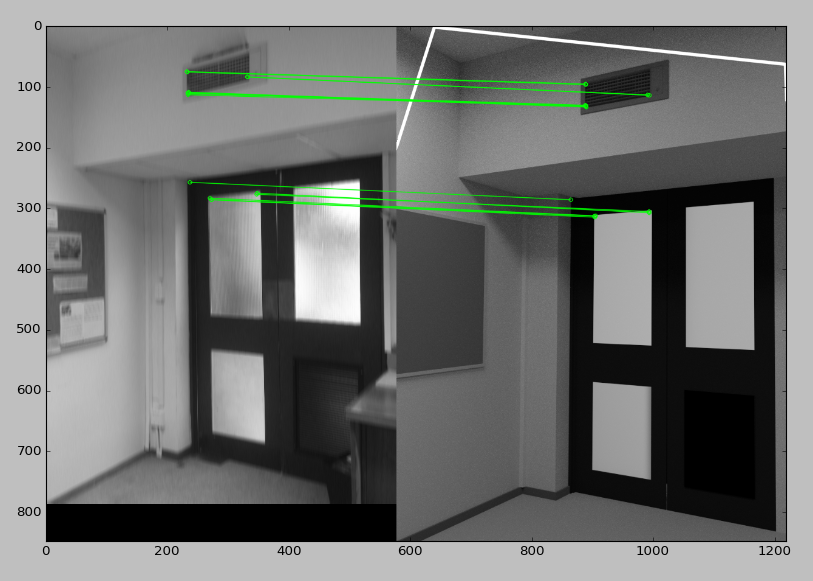
\includegraphics[width=1\textwidth]{y_blur}
						\caption{Blurring the photograph along the y axis}
						\label{fig:y_blur}
					\end{figure}
					
					Blurring the test image along the x direction slightly degraded the quality of the comparison. Blurring the test image along the y axis severely decreased the quality of the comparison.
					When blurring along either directions, the quality of the matches was not impaired, however there were significantly fewer matched features/key points when blurring along th y. The reason for this is not known.
					
				\paragraph{Edge detection}
					Performing edge detection on the test and query image produced very poor quality matches. A number of edge detection methods were employed using various settings, none of which produced any meaningful results.
					%TODO: Figure beolow was just for display purposes.
					As such, the figure \ref{fig:edge_detection_results} below of the edge detection comparison exists only to serve as an example of what edge detection produced.
					
					Features have been detected but have been poorly matched resulting in an overall poor comparison result.
					\begin{figure}[H]
						\centering
						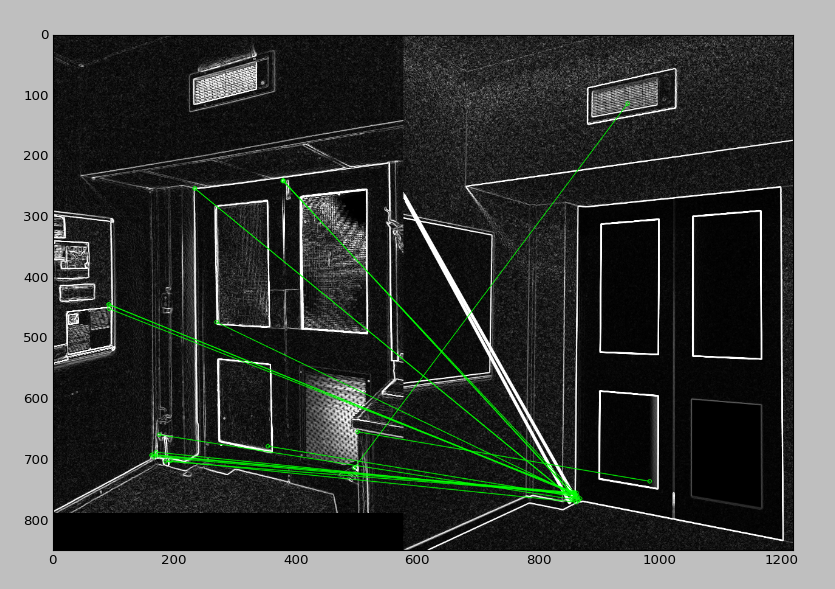
\includegraphics[width=1\textwidth]{edge_detection_results}
						\caption[Edge detection results]{Edge detection yielded poor results.}
						\label{fig:edge_detection_results}
					\end{figure}
					
			\subsubsection{Model adjustments}
				\paragraph{Level of detail}
					In figure \ref{fig:level_of_detail_results} the image of the air vent has been removed from the model, decreasing the level of detail of the model. The result was that there were fewer features/key points in total, and the matching of the features was poorer. From this it can be deduced that the higher the level of detail of the model, the higher the quality of the comparison, in terms of number of features found, as well as the quality of the matches.
					\begin{figure}[H]
						\centering
						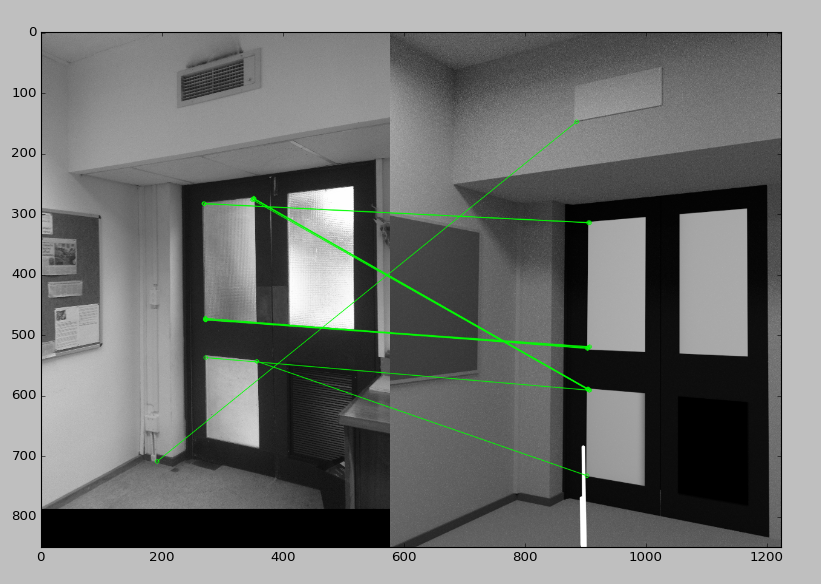
\includegraphics[width=1\textwidth]{level_of_detail_results}
						\caption[Level of detail results]{Decreasing the level of detail greatly reduced the quality of the comparison}
						\label{fig:level_of_detail_results}
					\end{figure}
				\paragraph{Lighting}
					Reducing the accuracy of the lighting yielded significantly poorer comparison results. To test the effect of lighting on the quality of the comparison process, the emmisive planes behind the doors were removed. From figure \ref{fig:reduced_lighting_results} it can be seen that the removal of the emmisive planes greatly reduced the number of features around the door section, however the features and matches on the air-conditioner vent were relatively unaffected. It can be deduced that the higher the accuracy and quality of lighting in the model, the higher the quality of comparison results.
					\begin{figure}[H]
						\centering
						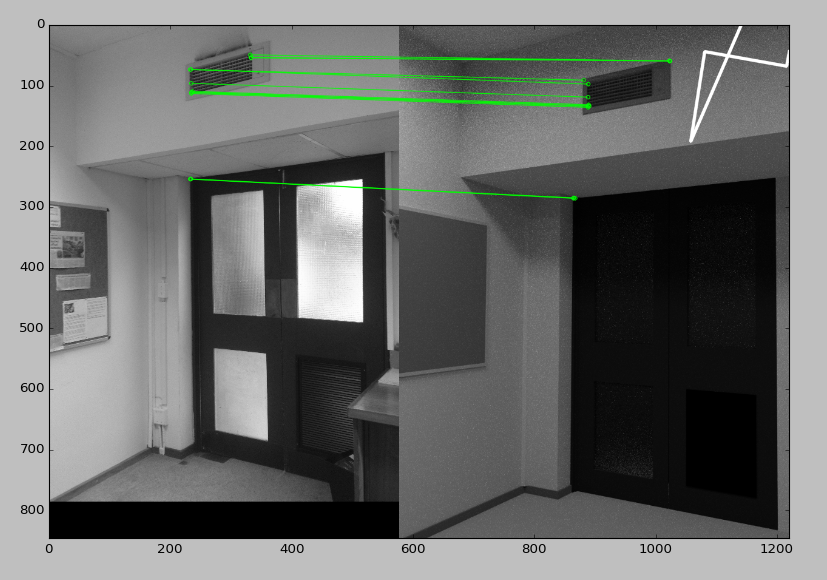
\includegraphics[width=1\textwidth]{reduced_lighting_results}
						\caption[Lighting results]{Decreasing the accuracy of the lighting yielded poorer results}
						\label{fig:reduced_lighting_results}
					\end{figure}
					
				\paragraph{Renders}
					Reducing the quality of the rendered image of the model greatly reduced the overall quality of the comparison result. The number of features was still relatively high, however the matches were of very poor quality. It can be deduced that the higher the quality of the render, the higher the quality of the comparison result.
					\begin{figure}[H]
						\centering
						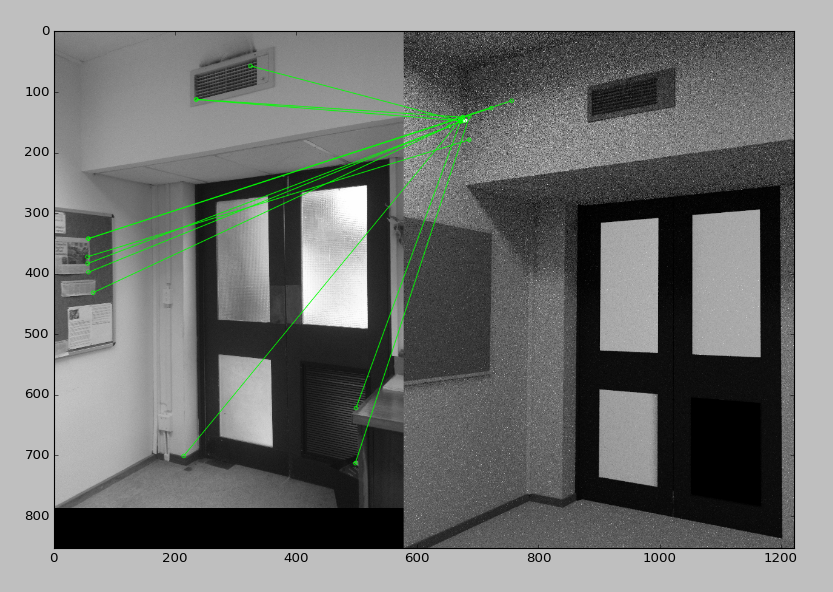
\includegraphics[width=1\textwidth]{low_quality_results}
						\caption[Render quality results]{Lower render quality produced poor comparison results.}
						\label{fig:low_quality_results}
					\end{figure}
				
			\subsubsection{Framework adjustments}
				\paragraph{Detectors}
					Two detectors were used in this investigation, the SIFT and ORB feature detector.
				\paragraph{Matchers}
					Two matchers were used in this investigation, the FLANN and Brute Force matchers.
				\paragraph{ORB and Brute Force}
					Using the ORB feature detector in combination with the Brute Force feature matcher yielded the highest quality comparison result. It is this result which served as the benchmark as stated in section \ref{benchmark}.
					\begin{figure}[H]
						\centering
						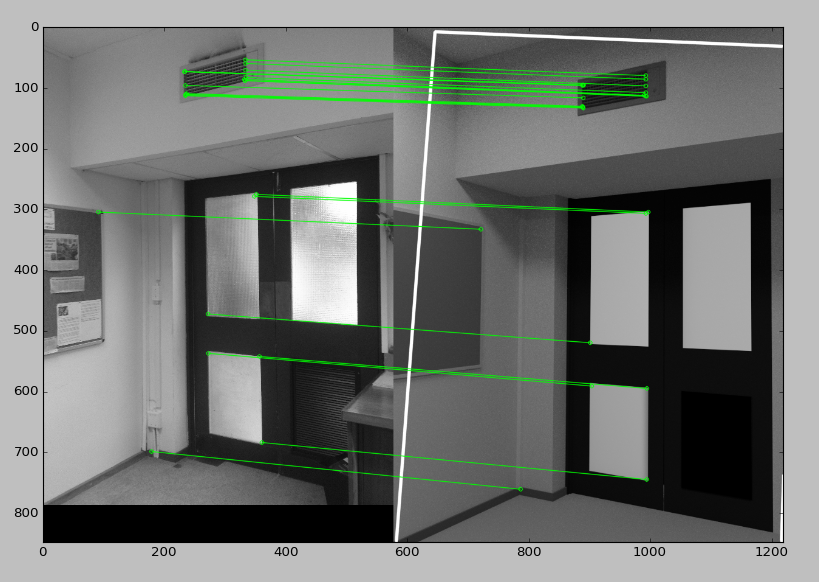
\includegraphics[width=1\textwidth]{best_comparason}
						\caption{ORB feature detector and Brute Force feature matcher.}
						\label{fig:orb_and_brute_force}
					\end{figure}
					
				\paragraph{ORB and FLANN}
					Due to various implementation details, using the ORB feature detector in combination with the FLANN feature matcher was not possible.
				
				\paragraph{SIFT and Brute Force}
					Due to various implementation details, using the SIFT feature detector in combination with the Brute Force feature matcher was not possible.
				
				\paragraph{SIFT and FLANN}
					Using the SIFT feature detector in combination with the FLANN feature matcher yielded mediocre comparison results. The result was that very few features were detected, however all the matches were of high quality.
					\begin{figure}[H]
						\centering
						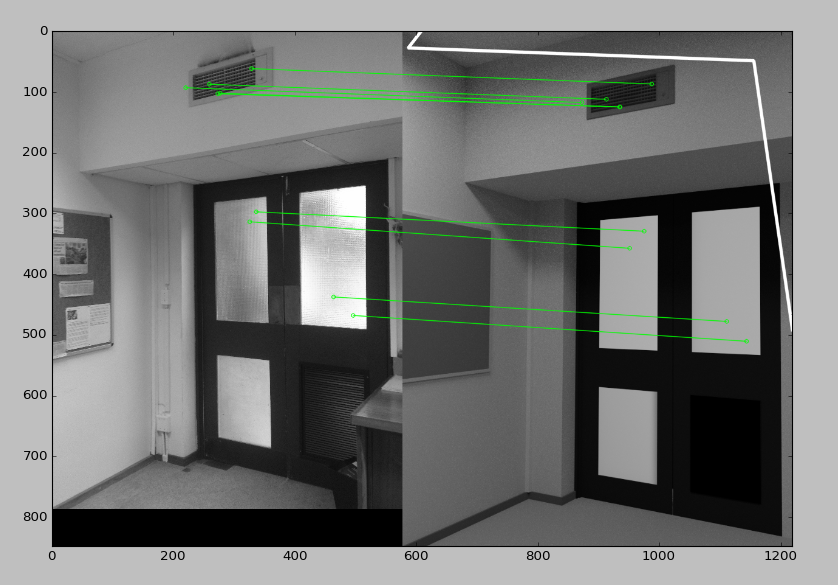
\includegraphics[width=1\textwidth]{sift_and_flann_results}
						\caption[SIFT and FLANN]{SIFT feature detector with FLANN feature matcher yielded a poor quality comparison result.}
						\label{fig:sift_and_flann_results}
					\end{figure}

\chapter{Discussions}
	\section{Quality of comparison}
	\label{comparison_quality}
		The quality of a comparison is determined by two factors, the number of matches, and the quality of the matches. The number of matches refers to the number of matched feature/key point pairs found in the comparison process. The quality of a match refers to the accuracy of a matched key point pair, basically the degree to which a matched key points represent the same real-world point. So a match would be of high quality if the key points of the match precisely represent the same real-world point.
		Determining and describing the quality of matches poses a problem, and that is that it is difficult to programmatically quantify the quality of a match. To get around this problem, matches have been visually inspected in order to determine their quality.

\chapter{Conclusions and future work}
	\section{Improving and furthering the investigation}
		\subsection{User Interface}
			A user interface could be created which would simplify the operation and usability of the testing framework. The user interface could be constructed using the QT graphical toolkit.
		
		\subsection{Further investigation}
			During the course of this investigation, many further potential investigative avenues have been discovered with regards to the comparison of photography and 3D models. The scope of this investigation has been continuously growing as the investigation progressed. Due to various constraints, not all of these avenues have been explored and there is much more to investigate.
		
	\section{Determining photographer's location}
		The main focus of this paper is on the comparison process between a photograph and a 3D model. What has not been discussed in great detail is how the comparison will enable the location of the photographer to be determined. These two problems have been separated due to the fact that the determination of the photographers location will not be possible without a sufficiently high quality comparison result. Given that the results of this investigation have indicated that a high quality comparison is realistically achievable, future work could include actually using the comparison results data in order to determine from where inside the 3D model the photograph was take. Two possible methods for achieving this are briefly introduced in the subsections below.
		
		\subsection{Geotagging renders}
			The most simple method of determining the photographers location would be to geotag each render of a series of renders of a 3D model. A photograph would then be compared against each render. The comparison with the highest quality will then be determined and the geotag of that render would indicate roughly where in the 3D model the photograph was taken, which would then sent to the photographer as their location.
			There are a number of implementation problems which exist, some of the main problems are worth mentioning here.
			The first problem is that as stated in section \ref{comparison_quality}, the quality of a comparison so far has not been able to be quantified. For the geotagging location method to be viable, a programmatic method of quantifying the quality of a comparison is needed.
			Another problem is that of geotagging renders. This process needs to be done automatically in order to be viable.
			
		\subsection{Photogrammetric principles}
			Another method for determining the photographers location involves making use of photogrammetric principles. Using the collinearity equations, a resection can be performed to determine the location of the camera.
			\begin{figure}[H]
				\centering
				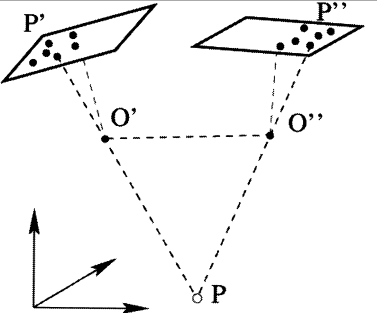
\includegraphics[width=1\textwidth]{collinearity_equations}
				\caption[Collinearity Equations]{Collinearity equations can be used to determine a photographers position.}
				\label{fig:collinearity_equations}
			\end{figure}
			
	\section{Conclusions}
		Based on the results above, it is possible to compare a photograph to a 3D model by creating renderings of the model and using image comparison software compare photographs to renders of a 3D model.
		
		It is clear that the accuracy of the model and the quality of a comparison is positively correlated, that is that the greater the quality and accuracy of the model, the higher the quality of the comparison.
		
\newpage

%\printbibliography
\addcontentsline{toc}{chapter}{Bibliography}
\bibliography{sources} % This command creates the bibliography

\end{document}